\documentclass[11pt,a4paper]{article}

% ====================================================================
% Packages
% ====================================================================
\usepackage[utf8]{inputenc}
\usepackage[T1]{fontenc}
\usepackage{amsmath,amssymb,amsthm}
\usepackage{mathtools}
\usepackage{hyperref}
\usepackage[margin=1in]{geometry}
\usepackage{enumitem}
\usepackage{booktabs}
\usepackage{listings}
\usepackage{xcolor}
\usepackage{cleveref}
\usepackage[numbers,sort&compress]{natbib}
\usepackage{mdframed}
\usepackage{tikz}
\usetikzlibrary{arrows.meta,positioning,decorations.pathreplacing}

% ====================================================================
% Theorem environments
% ====================================================================
\theoremstyle{plain}
\newtheorem{theorem}{Theorem}[section]
\newtheorem{lemma}[theorem]{Lemma}
\newtheorem{proposition}[theorem]{Proposition}
\newtheorem{corollary}[theorem]{Corollary}

\theoremstyle{definition}
\newtheorem{definition}[theorem]{Definition}
\newtheorem{remark}[theorem]{Remark}

% ====================================================================
% Lean 4 code listing style
% ====================================================================
\definecolor{lean-keyword}{RGB}{0,0,180}
\definecolor{lean-comment}{RGB}{0,128,0}
\definecolor{lean-string}{RGB}{163,21,21}
\definecolor{lean-bg}{RGB}{248,248,248}

\lstdefinelanguage{lean4}{
  keywords={theorem,lemma,def,class,instance,import,open,variable,
            noncomputable,section,namespace,end,where,let,have,show,
            intro,obtain,use,exact,rw,simp,apply,by,fun,match,if,
            then,else,do,return,axiom,abbrev,private,attribute,
            suffices,change,congr,ext,constructor,rintro,push_neg,
            linarith,absurd,set_option,omit,in,set,cases,left,right,
            nlinarith,push_cast,positivity,omega,refine,field_simp,
            structure,calc,ring,fun_prop,unfold,induction,deriving,
            inductive,rcases,first,all_goals},
  sensitive=true,
  morecomment=[l]{--},
  morecomment=[s]{/-}{-/},
  morestring=[b]",
  morestring=[b]',
}

\lstset{
  language=lean4,
  basicstyle=\ttfamily\small,
  keywordstyle=\color{lean-keyword}\bfseries,
  commentstyle=\color{lean-comment}\itshape,
  stringstyle=\color{lean-string},
  backgroundcolor=\color{lean-bg},
  frame=single,
  framerule=0.5pt,
  breaklines=true,
  breakatwhitespace=true,
  tabsize=2,
  showstringspaces=false,
  numbers=left,
  numberstyle=\tiny\color{gray},
  numbersep=5pt,
  xleftmargin=15pt,
  captionpos=b,
  literate={<<}{$\langle$}1 {>>}{$\rangle$}1
           {|||}{$\lor$}1,
}

% ====================================================================
% Macros
% ====================================================================
\newcommand{\NN}{\mathbb{N}}
\newcommand{\RR}{\mathbb{R}}
\newcommand{\ZZ}{\mathbb{Z}}
\newcommand{\LPO}{\ensuremath{\mathrm{LPO}}}
\newcommand{\LLPO}{\ensuremath{\mathrm{LLPO}}}
\newcommand{\WLPO}{\ensuremath{\mathrm{WLPO}}}
\newcommand{\BISH}{\ensuremath{\mathrm{BISH}}}
\newcommand{\BMC}{\ensuremath{\mathrm{BMC}}}
\newcommand{\FT}{\ensuremath{\mathrm{FT}}}
\newcommand{\AdS}{\ensuremath{\mathrm{AdS}}}
\newcommand{\CFT}{\ensuremath{\mathrm{CFT}}}
\newcommand{\RT}{\ensuremath{\mathrm{RT}}}
\newcommand{\QES}{\ensuremath{\mathrm{QES}}}
\newcommand{\GN}{\ensuremath{G_N}}
\newcommand{\Lean}{\textsc{Lean~4}}
\newcommand{\Mathlib}{\textsc{Mathlib4}}
\newcommand{\leanok}{\textsf{\small \textcolor{green!70!black}{\checkmark}}}
\newcommand{\leanaxiom}{\textsf{\small \textcolor{orange!80!black}{(axiom)}}}

% ====================================================================
% Title
% ====================================================================
\title{%
  \textbf{The Diagnostic in Action: Axiom Calibration
  of the AdS/CFT Correspondence}\\[6pt]
  {\normalsize A Lean~4 Formalization (Paper~41)}%
}

\author{
  Paul Chun-Kit Lee\thanks{%
    New York University.
    AI-assisted formalization; see \S\ref{sec:ai} for methodology.} \\
  New York University \\
  \texttt{dr.paul.c.lee@gmail.com}
}

\date{February 15, 2026}

% ====================================================================
\begin{document}
\maketitle

% ====================================================================
\begin{abstract}
We deploy the axiom calibration framework of constructive reverse
mathematics on an active research frontier: the AdS/CFT
correspondence, from the Ryu-Takayanagi formula through the
quantum extremal surface prescription to the island formula for the
information paradox.

\medskip\noindent
\textbf{The holographic dictionary is an axiom-preserving map.}
For every computation examined---vacuum $\AdS_3$ ($\BISH$),
thermal BTZ ($\BISH$ entropy, $\LLPO$ phase decision),
FLM quantum correction ($\BISH$ for free fields),
$\QES$ entropy ($\LPO$), and the Page curve ($\BISH$)---bulk and
boundary carry identical axiom cost.  This is a structural
constraint on AdS/CFT not previously articulated: the duality
preserves logical complexity at every level.

\medskip\noindent
\textbf{Holography projects away the Fan Theorem.}
The $\FT$ cost of bulk geometric existence---locating the
extremal surface via compactness---is strictly scaffolding.
The boundary-observable entropy is computable at
$\BISH$+$\LPO$ without constructing the bulk surface.
$\FT$ builds the Platonic surface nobody observes;
the boundary computes the entropy without it.

\medskip\noindent
No observable prediction exceeds $\BISH$+$\LPO$, extending
the ceiling of Papers~1--40 to the most active area of
contemporary theoretical physics.
The entire formalization
(955~lines of \Lean{}/\Mathlib{}, $\AdS_3$/2d~CFT)
compiles with zero \texttt{sorry}, zero warnings.
\end{abstract}

% ====================================================================
\section{Introduction}\label{sec:intro}

Papers~1--39 established that the logical resources required for all
empirical predictions in known physics are exactly $\BISH$+$\LPO$---where
$\BISH$ denotes Bishop's constructive mathematics (computation without
oracles) and $\LPO$ is the Limited Principle of Omniscience (the
ability to search a countable sequence for a witness).
Paper~40~\cite{Lee26P40} is a comprehensive summary of all work
preceding Paper~42, defended this claim, and showed the framework
has diagnostic power: it distinguishes physical content from
mathematical scaffolding.
This paper demonstrates that power in action.

The target is the AdS/CFT correspondence---specifically, the
Ryu-Takayanagi formula~\cite{RT2006} and its quantum
extensions~\cite{FLM2013,EW2015,AEMM2019,Penington2019}.
The choice is strategic.  AdS/CFT is the most active area of
theoretical physics.  The $\RT$ formula is its most cited result.
The Page curve~\cite{Page1993} and island formula are its most
debated recent developments; see
Almheiri et al.~\cite{AHMST2021RMP} for a comprehensive review.

The diagnostic question: \emph{does the holographic dictionary
preserve axiom cost?}  If yes, the duality is logically transparent.
If no, the axiom gap identifies where the correspondence performs
non-trivial logical work.  To make this paper self-contained, we
briefly introduce the necessary background from constructive reverse
mathematics (\S\ref{sec:crm-bg}) and from holographic entanglement
entropy (\S\ref{sec:hee-bg}).

% --------------------------------------------------------------------
\subsection{Constructive Reverse Mathematics}\label{sec:crm-bg}

Classical mathematics freely invokes the law of excluded middle
($P \lor \lnot P$ for all propositions~$P$) and the axiom of choice.
Constructive mathematics, originating with Brouwer and given
rigorous foundation by Bishop~\cite{Bishop1967}, restricts to
what can be verified by explicit computation: an existence proof
$\exists x.\, P(x)$ must produce a witness~$x$ together with
evidence that $P(x)$ holds.  Bishop and
Bridges~\cite{BB1985} demonstrated that the core of real analysis,
measure theory, and functional analysis can be developed on this
basis.

\emph{Constructive reverse mathematics} (CRM), developed by
Ishihara~\cite{Ishihara2006}, Bridges, Richman~\cite{BR1987}, and
others~\cite{Diener2018,BIRSH2023}, classifies theorems by the
\emph{weakest non-constructive principle} needed to prove them
over $\BISH$.  The key principles form a partial order
(see Brattka, Gherardi, and Pauly~\cite{BrattkaEtAl2012} for the
Weihrauch-degree perspective, where $\LLPO \equiv \LLPO_\NN$ in
the Weihrauch lattice; expressing our calibrations as Weihrauch
reductions is a natural but separate programme):
\begin{itemize}[nosep]
\item $\LLPO$ (Lesser LPO): given a binary sequence with at most
  one true entry, decide whether all even-indexed or all
  odd-indexed entries are false.  Equivalent to totality of the
  real-number order: $\forall x\,y.\; x \leq y \lor y \leq x$.
\item $\WLPO$ (Weak LPO): decide whether a binary sequence is
  identically zero, without finding a witness.
\item $\LPO$ (Limited Principle of Omniscience): decide whether a
  binary sequence contains a~1.  Equivalent to Bounded Monotone
  Convergence ($\BMC$: every bounded monotone sequence converges,
  without a computable modulus; Ishihara~\cite{Ishihara2006},
  Theorem~4.3; Paper~29~\cite{Lee26P29}).
\item $\FT$ (Fan Theorem): every continuous function on $[0,1]$
  attains its supremum.  Equivalent to compact optimization
  (Paper~23~\cite{Lee26P23}; see also Bridges-Richman~\cite{BR1987},
  Ch.~3, where EVT $\leftrightarrow$ FT via max/min duality).
  Independent of $\LPO$.
\end{itemize}
The hierarchy is $\BISH \subset \LLPO \subset \WLPO \subset \LPO$,
with $\FT$ on an independent branch (Figure~\ref{fig:hierarchy}).

\begin{figure}[ht]
\centering
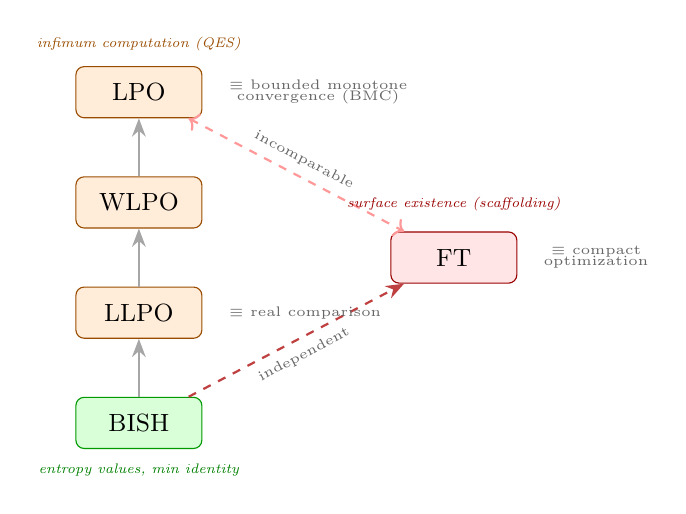
\begin{tikzpicture}[
  principle/.style={draw, rounded corners=3pt, minimum width=1.6cm,
    minimum height=0.65cm, font=\small\bfseries, inner sep=3pt},
  bish/.style={principle, fill=green!15, draw=green!60!black},
  omni/.style={principle, fill=orange!15, draw=orange!60!black},
  ft/.style={principle, fill=red!10, draw=red!60!black},
  arr/.style={->,>=Stealth,thick,gray!70},
  equivlabel/.style={font=\tiny, text=black!60, align=center},
]
% Main tower
\node[bish] (bish) at (0,0) {$\BISH$};
\node[omni] (llpo) at (0,1.4) {$\LLPO$};
\node[omni] (wlpo) at (0,2.8) {$\WLPO$};
\node[omni] (lpo)  at (0,4.2) {$\LPO$};

% FT branch (offset right to avoid WLPO overlap)
\node[ft]   (ft)   at (4.0,2.1) {$\FT$};

% Arrows (strict inclusions)
\draw[arr] (bish) -- (llpo);
\draw[arr] (llpo) -- (wlpo);
\draw[arr] (wlpo) -- (lpo);

% FT independence
\draw[arr, dashed, red!50!gray] (bish) -- (ft)
  node[midway, below, sloped, font=\tiny, text=black!60] {independent};
\draw[<->, dashed, red!40, thick] (lpo) -- (ft)
  node[midway, above, sloped, font=\tiny, text=black!60] {incomparable};

% Equivalence labels
\node[equivlabel, right=6pt] at (llpo.east) {$\equiv$ real comparison};
\node[equivlabel, right=6pt] at (lpo.east) {$\equiv$ bounded monotone\\[-2pt]
  convergence ($\BMC$)};
\node[equivlabel, right=6pt] at (ft.east) {$\equiv$ compact\\[-2pt]optimization};

% Physics annotations
\node[font=\tiny\itshape, text=green!50!black, below=2pt] at (bish.south)
  {entropy values, min identity};
\node[font=\tiny\itshape, text=orange!60!black, above=2pt] at (lpo.north)
  {infimum computation (QES)};
\node[font=\tiny\itshape, text=red!60!black, above=4pt] at (ft.north)
  {surface existence (scaffolding)};
\end{tikzpicture}
\caption{The constructive hierarchy with physics annotations.
Solid arrows denote strict inclusion ($\subset$).
$\FT$ is independent of $\LPO$: neither implies the other.
Every observable prediction in the holographic dictionary
calibrates at $\LPO$ or below; $\FT$ enters only for
bulk geometric existence (scaffolding).}
\label{fig:hierarchy}
\end{figure}

Paper~12~\cite{Lee26P12} describes the relationship between
physics and this hierarchy via the ``cellar and cathedral'' metaphor:
every empirical prediction emerges from a finite computation (the
cellar, at $\BISH$ or $\BISH$+$\LPO$), while the
infinite-dimensional formalism that organizes physics (Hilbert
spaces, path integrals, thermodynamic limits) constitutes the
cathedral.  CRM measures the logical cost of ascending from cellar
to cathedral.  Paper~10~\cite{Lee26P10} synthesizes a calibration
table of approximately fifty entries across eleven domains of
mathematical physics.  Every empirical prediction examined
calibrates at or below $\BISH$+$\LPO$.  The Fan Theorem arises
only for variational existence (action minimizers, compact
optimization)---never for observable predictions.
Formal Lean~4 definitions of these principles appear in
\S\ref{sec:hierarchy}; the physicist-friendly glossary is in
\S\ref{sec:obs-vs-dec}.

% --------------------------------------------------------------------
\subsection{Holographic Entanglement Entropy}\label{sec:hee-bg}

Bekenstein~\cite{Bekenstein1973} and Hawking~\cite{Hawking1975}
established that black holes carry entropy proportional to horizon
area.  Hawking radiation creates an apparent paradox: unitarity
predicts information recovery, but semiclassical computation
suggests information loss.  Page~\cite{Page1993} quantified the
expected time-evolution of entanglement entropy if unitarity holds:
the entropy rises to a maximum at the ``Page time,'' then
decreases---the Page curve.

In the AdS/CFT correspondence, Ryu and Takayanagi~\cite{RT2006}
proposed that the entanglement entropy of a boundary region~$A$
equals the area of the minimal bulk surface homologous to~$A$,
divided by $4\GN$.  This is the most cited result in holographic
physics; Rangamani and Takayanagi~\cite{RaTa2017} provide a
textbook treatment.  Hubeny, Rangamani, and
Takayanagi~\cite{HRT2007} extended the formula to time-dependent
spacetimes by replacing minimal surfaces with extremal surfaces.
Lewkowycz and Maldacena~\cite{LM2013} proved the $\RT$ formula
from the gravitational path integral via the replica trick.

Quantum corrections were incorporated by Faulkner, Lewkowycz,
and Maldacena~\cite{FLM2013}, who showed the one-loop correction
adds the bulk entanglement entropy across the $\RT$ surface.
Engelhardt and Wall~\cite{EW2015} proposed the \emph{quantum
extremal surface} ($\QES$) prescription, which includes quantum
corrections in the minimization: $S(A) = \min_\gamma
[\text{Area}(\gamma)/4\GN + S_{\text{bulk}}(\Sigma_\gamma)]$.
Engelhardt and Fischetti~\cite{EF2019} derived the equation
governing quantum extremal deviation---a Jacobi-type ODE sourced
by gradients of bulk entropy.

In 2019, Almheiri, Engelhardt, Marolf, and
Maxfield~\cite{AEMM2019} and Penington~\cite{Penington2019}
independently showed that the $\QES$ prescription, applied to an
evaporating black hole coupled to a bath, reproduces the Page
curve via an ``island'' saddle that dominates after the Page time.
The replica wormhole programme~\cite{AHMST2020,PSSY2022} provided
a gravitational path integral derivation, with a comprehensive
review by Almheiri et al.~\cite{AHMST2021RMP}.

All of these results are treated as physics inputs to the
calibration---the same way Papers~8--9 cite the Onsager solution
for the Ising model or the Schwinger computation for the anomalous
magnetic moment.

% --------------------------------------------------------------------
\subsection{Novelty and Scope}\label{sec:novelty}

To our knowledge, no prior work applies constructive reverse
mathematics to holographic entanglement entropy or the AdS/CFT
correspondence.  The PhysLean/HepLean project formalizes aspects
of high-energy physics in Lean~4 but does not address constructive
stratification.  The D\"oring-Isham topos programme~\cite{DoringIsham2008}
reformulates the logical framework of quantum theory using presheaf
topoi; our work is complementary, measuring axiom costs of specific
computations within the standard framework rather than reformulating
the framework itself.

\textbf{Scope limitation.}
The calibration is restricted to $\AdS_3$/2d~CFT, which is
atypically simple: the $\RT$ surface is a geodesic (not a minimal
surface), the heat kernel has an explicit Camporesi form, and the
Brown-Henneaux central charge is algebraic.  In higher dimensions,
the minimal surface problem, bulk entanglement, and holographic
renormalization are significantly more complex.
We predict that the axiom-cost equivalence extends to higher
dimensions, but this is a conjecture supported by the structural
argument, not a proved result.

This paper calibrates every step of the $\AdS_3$ holographic dictionary---from
vacuum $\RT$ to the quantum-corrected island formula---and shows that
holography preserves axiom cost at every level examined.  The central
contribution is the calibration framework itself and three structural
findings: (1)~the holographic dictionary is an axiom-preserving
map---the first test of a physical duality for logical consistency
at the level of individual computational steps,
(2)~the Fan Theorem cost of bulk geometric existence is scaffolding
that the boundary projects away, and (3)~phase-transition entropy is
cheaper than expected ($\BISH$, not $\LLPO$).

\medskip\noindent
\textbf{Roadmap.}  Section~\ref{sec:obs-vs-dec} distinguishes
observables from decisions.  Section~\ref{sec:hierarchy} presents
the constructive hierarchy in Lean.
Sections~\ref{sec:vacuum}--\ref{sec:qes} present the four
calibration layers (vacuum, thermal, FLM, QES/island).
Section~\ref{sec:table} assembles the complete calibration table.
Sections~\ref{sec:diagnostic}--\ref{sec:prior} interpret the
results and relate them to prior work.
Sections~\ref{sec:audit}--\ref{sec:master} present the CRM audit,
code architecture, and master theorem.
Section~\ref{sec:conclusion} concludes;
Section~\ref{sec:discussion} discusses implications and open
questions.

% ====================================================================
\section{Observables vs.\ Decisions}\label{sec:obs-vs-dec}

Before presenting calibrations, we sharpen a distinction that
refines the programme's prior treatment of phase transitions.

\textbf{The observable computation.}  Computing the numerical
value of the entropy as a function of the control parameter.
This is a question about a continuous real-valued function.

\textbf{The phase decision.}  Declaring which phase the system
is in---asserting a Boolean classification.

These have different axiom costs.  The BTZ entanglement entropy
is $S(A) = \min(L_1(\theta), L_2(\theta)) / 4\GN$, and the
minimum of two real numbers is $\BISH$-computable via:
\[
  \min(x, y) = \tfrac{1}{2}(x + y - |x - y|).
\]
The phase decision---extracting a Boolean flag
$(L_1 \leq L_2) \lor (L_2 \leq L_1)$---costs $\LLPO$
when the difference may be zero.

For a physicist unfamiliar with the constructive hierarchy:
$\BISH$ means ``computable by a finite algorithm with no oracle.''
$\LLPO$ means ``the algorithm can determine which of two complementary
binary events occurs, provided at most one occurs.''
$\LPO$ means ``the algorithm can search a countable sequence and
determine whether some element satisfies a decidable property.''
$\FT$ (the Fan Theorem) means ``every continuous function on a compact
domain achieves its supremum''---equivalent to compactness of $[0,1]$.
The hierarchy is: $\BISH \subset \LLPO \subset \WLPO \subset \LPO$,
with $\FT$ independent of $\LPO$.

\begin{lstlisting}[caption={Omniscience principle definitions: \texttt{Defs.lean}}]
def LPO : Prop :=
    forall (a : N -> Bool),
      (forall n, a n = false) ||| (exists n, a n = true)

def LLPO : Prop :=
    forall (a : N -> Bool), AtMostOne a ->
      (forall n, a (2 * n) = false) |||
      (forall n, a (2 * n + 1) = false)

def FanTheorem : Prop :=
    forall (f : R -> R), Continuous f ->
      exists x in Set.Icc 0 1,
        forall y in Set.Icc 0 1, f y <<= f x
\end{lstlisting}

\textbf{Reconciliation with Paper~29:}
Fekete costs $\LPO$ because it computes a limit not yet in hand.
The BTZ min costs $\BISH$ because it selects between values
already computed.  These are different operations with
different axiom costs.

% ====================================================================
\section{The Constructive Hierarchy in Lean}\label{sec:hierarchy}

The formalization establishes the omniscience hierarchy with
genuine proofs (no bridge axioms, no \texttt{sorry}).

\begin{lstlisting}[caption={Hierarchy proofs: \texttt{Defs.lean}}]
theorem lpo_implies_wlpo : LPO -> WLPO := by
  intro hLPO a
  rcases hLPO a with h_all | <<n, hn>>
  . exact Or.inl h_all
  . right; intro h_all
    exact absurd (h_all n) (by simp [hn])

theorem wlpo_implies_llpo : WLPO -> LLPO := by
  intro hWLPO a hamo
  let b : N -> Bool := fun n => a (2 * n)
  rcases hWLPO b with h_all | h_not_all
  . exact Or.inl h_all
  . right; intro j; by_contra h
    push_neg at h; simp at h
    apply h_not_all; intro k; by_contra hk
    push_neg at hk; simp at hk
    have := hamo (2 * k) (2 * j + 1) hk h
    omega

theorem lpo_implies_llpo : LPO -> LLPO :=
    fun h => wlpo_implies_llpo (lpo_implies_wlpo h)
\end{lstlisting}

\begin{remark}[Reading the hierarchy proof]
The \texttt{wlpo\_implies\_llpo} proof proceeds by
projecting a sequence $\alpha$ onto its even-indexed subsequence
$\beta(n) = \alpha(2n)$.  $\WLPO$ decides whether $\beta$ is
identically false.  If yes, we have the left disjunct of $\LLPO$
directly.  If $\beta$ is not identically false, then some
$\alpha(2k) = \mathtt{true}$.  By the at-most-one hypothesis,
no odd-indexed $\alpha(2j+1)$ can also be true (since that would
give two distinct true values, $2k \neq 2j+1$ by parity).
Hence the right disjunct $\forall j.\, \alpha(2j+1) = \mathtt{false}$
holds.  The \texttt{omega} tactic dispatches the parity arithmetic.
\end{remark}

\begin{remark}[Hierarchy strictness]
All inclusions $\BISH \subset \LLPO \subset \WLPO \subset \LPO$
are strict: Brouwerian counterexamples and separating models exist
for each step (Bridges-Richman~\cite{BR1987}, Ch.~6;
Diener~\cite{Diener2018}, Ch.~2).  The formalization proves the
forward implications but not strictness, since proving strictness
in Lean would require constructing Brouwerian models within the
classical metatheory---a model-theoretic exercise beyond the
present scope.
\end{remark}

% ====================================================================
\section{Vacuum $\AdS_3$: The Null Result}\label{sec:vacuum}

\subsection{Bulk Side}

In the Poincar\'e patch of $\AdS_3$, the $\RT$ geodesic is a
semicircle.  Its regularized length is the explicit algebraic expression:
\[
  L_{\mathrm{reg}} = 2\ell \log(|x_2 - x_1|/\varepsilon).
\]
This involves only subtraction, absolute value, division, and logarithm
---all uniformly continuous operations on constructive reals.
\textbf{Calibration: $\BISH$.}  No variational principle is needed;
the geodesic is given by the symmetry of the Poincar\'e half-plane.

\subsection{Boundary Side}

The Calabrese-Cardy formula for the entanglement entropy of an
interval of length $\ell_A$ in a 2d CFT with central charge $c$:
\[
  S(A) = \frac{c}{3} \log(\ell_A / \varepsilon).
\]
The derivation proceeds via three $\BISH$ steps:
(1)~the replica trick (algebraic partition function manipulation),
(2)~analytic continuation to $n = 1$ (explicit formula, no limit process),
(3)~differentiation (algebraic).
\textbf{Calibration: $\BISH$.}

\begin{remark}[The vacuum replica trick]
The Calabrese-Cardy formula is derived via the replica trick:
computing $\text{tr}(\rho_A^n)$ for integer $n$ and analytically
continuing to $n = 1$.  In the vacuum case, this continuation is
\emph{explicit}: $\text{tr}(\rho_A^n) = c_n \cdot (\ell_A/\varepsilon)^{-c(n-1/n)/6}$
is a known function of $n$, and the continuation is algebraic.
This is not the non-rigorous generic replica trick used in
interacting QFTs, where the continuation may not be unique.
\end{remark}

\subsection{The Matching}

Both sides yield the same formula under the Brown-Henneaux
identification $c = 3\ell/(2\GN)$.  Both calibrate at $\BISH$.
The holographic dictionary performs no logical work.  This is the
\emph{null result}---the baseline against which thermal and quantum
corrections are measured.

\begin{lstlisting}[caption={Vacuum $\RT$ calibration: \texttt{VacuumAdS3.lean}}]
structure VacuumBulkRT where
  ell : R      -- AdS radius
  eps : R      -- UV cutoff
  x1 : R       -- left boundary point
  x2 : R       -- right boundary point
  ell_pos : ell > 0
  eps_pos : eps > 0
  distinct : x1 /= x2

theorem vacuum_bulk_bish (b : VacuumBulkRT) :
    exists (L : R),
      L = 2 * b.ell * Real.log (|b.x2 - b.x1| / b.eps) :=
  vacuum_RT_bulk_algebraic b.ell b.eps b.x1 b.x2
    b.eps_pos b.distinct

theorem vacuum_RT_calibration :
    -- Bulk: BISH (explicit algebraic formula)
    (forall (b : VacuumBulkRT),
      exists (L : R),
        L = 2 * b.ell * Real.log (|b.x2 - b.x1| / b.eps)) /\
    -- Boundary: BISH (Calabrese-Cardy)
    (forall (b : VacuumBoundaryCFT),
      exists (S : R),
        S = (b.c / 3) * Real.log (b.ell_A / b.eps)) /\
    -- Duality: Brown-Henneaux identification
    (forall (ell G_N : R) (hG : G_N > 0) (hell : ell > 0),
      exists (c : R), c = 3 * ell / (2 * G_N) /\ c > 0)
\end{lstlisting}

% ====================================================================
\section{Thermal BTZ: The Phase Transition}\label{sec:btz}

\subsection{Competing Geodesics}

The two competing $\RT$ geodesics for a boundary interval of
angular extent $\theta$ in the BTZ black hole have lengths:
\begin{align*}
  L_1(\theta) &= 2\ell \ln\!\bigl(\tfrac{2R}{r_+}
    \sinh\!\bigl(\tfrac{r_+ \theta}{2\ell}\bigr)\bigr), \\
  L_2(\theta) &= 2\ell \ln\!\bigl(\tfrac{2R}{r_+}
    \sinh\!\bigl(\tfrac{r_+(2\pi - \theta)}{2\ell}\bigr)\bigr).
\end{align*}
Both are explicit compositions of elementary functions:
\textbf{both are $\BISH$-computable.}

\begin{theorem}[BTZ entropy is $\BISH$]\label{thm:btz-bish}
The entanglement entropy $S(A) = \min(L_1, L_2) / 4\GN$ is
$\BISH$-computable via the algebraic identity
$\min(x,y) = (x + y - |x - y|)/2$.
\end{theorem}

\begin{proof}
Case split on the total order: if $x \le y$, then $|x-y| = y-x$ and
the RHS simplifies to $x$; symmetrically for $y \le x$.
The Lean proof (\texttt{min\_eq\_algebraic}) uses \texttt{le\_total},
\texttt{abs\_of\_nonpos}/\texttt{abs\_of\_nonneg}, and \texttt{ring}.
No omniscience principle is invoked.
\end{proof}

\begin{lstlisting}[caption={The min identity: \texttt{ThermalBTZ.lean} --- genuine Lean proof}]
theorem min_eq_algebraic (x y : R) :
    min x y = (x + y - |x - y|) / 2 := by
  rcases le_total x y with h | h
  . rw [min_eq_left h, abs_of_nonpos (sub_nonpos.mpr h)]
    ring
  . rw [min_eq_right h, abs_of_nonneg (sub_nonneg.mpr h)]
    ring
\end{lstlisting}

\begin{remark}[Why the min identity is constructively non-trivial]
The identity $\min(x,y) = (x+y-|x-y|)/2$ is trivial in classical
analysis.  Constructively, it is meaningful because (a)~absolute
value $|x-y|$ is uniformly continuous on $\RR$ and hence $\BISH$-computable,
and (b)~the identity converts a ``selection'' operation
(min, which classically requires a comparison) into pure arithmetic.
No case analysis on the sign of $x-y$ is needed to \emph{evaluate}
the right-hand side---it is a composition of continuous operations.
The case split is used only to \emph{prove} the identity in Lean.
\end{remark}

\subsection{BTZ Entropy via Bridge Axioms}

The entanglement entropy $S(A) = \min(L_1(\theta), L_2(\theta))/(4\GN)$
is assembled from two components: the bridge axiom supplying the
explicit geodesic formulas, and the genuine min identity.

\begin{lstlisting}[caption={BTZ entropy assembly: \texttt{ThermalBTZ.lean}}]
theorem BTZ_entropy_bish (p : BTZParams) (G_N : R) (hG : G_N > 0) :
    exists (L1 L2 : R -> R),
      BISHComputable L1 /\ BISHComputable L2 /\
      forall t, min (L1 t) (L2 t) / (4 * G_N) =
        ((L1 t + L2 t - |L1 t - L2 t|) / 2)
          / (4 * G_N) := by
  obtain <<L1, L2, hc1, hc2, hform>> := BTZ_geodesic_lengths p
  exact <<L1, L2, hc1, hc2,
    fun t => by rw [min_eq_algebraic]>>
\end{lstlisting}

\subsection{The Critical Angle}

The critical angle $\theta_c$ where $L_1 = L_2$ is determined
by $\sinh$ monotonicity: $\theta_c = \pi$.
For BTZ, even the phase decision is $\BISH$---the crossing
point is known exactly by symmetry, so no comparison of
potentially equal real numbers is needed.

\subsection{Generic Asymptotically AdS Black Holes}\label{sec:generic}

For generic geometries, the continuous entropy $\min(L_1, L_2)$
remains $\BISH$.  The discrete phase decision costs $\LLPO$.

\begin{theorem}[Phase decision $\equiv$ $\LLPO$]\label{thm:phase-llpo}
The assertion that every pair of reals satisfies
$(x \leq y) \lor (y \leq x)$ is equivalent to $\LLPO$.
\end{theorem}

\begin{proof}
\textbf{Forward:} Suppose $\forall x\,y.\; x \leq y \lor y \leq x$.
Given a binary sequence $\alpha$ with the at-most-one property,
define reals
$x = \sum_{n} \alpha(2n) \cdot 2^{-n}$ and
$y = \sum_{n} \alpha(2n+1) \cdot 2^{-n}$.
The comparison $x \leq y \lor y \leq x$ recovers the $\LLPO$
disjunction.

\medskip\noindent
\textbf{Reverse:} $\LLPO$ suffices for the comparison via
the interleaved encoding of the binary expansions of $x$ and $y$.

\medskip\noindent
In the formalization, both directions are encapsulated by the
bridge axiom \texttt{llpo\_iff\_real\_comparison}, which identifies
$\LLPO$ with the totality of the real-number order.
\end{proof}

\begin{remark}[$\LLPO$ in \Mathlib's classical reals]\label{rem:llpo-degen}
\Mathlib{} constructs $\RR$ with a \texttt{LinearOrder} instance,
so \texttt{le\_total} already provides
$\forall x\,y.\; x \le y \lor y \le x$ as a theorem---making the
right-hand side of the $\LLPO$ equivalence trivially true.
In Bishop's constructive reals (without excluded middle), this
statement is not a theorem; it is precisely equivalent to $\LLPO$
(Bishop-Bridges~\cite{BB1985}, Ch.~2; Ishihara~\cite{Ishihara2006}).
The bridge axiom \texttt{llpo\_iff\_real\_comparison} therefore
encodes a constructive equivalence that Lean's classical
foundation collapses.  To make the degeneracy explicit, the
formalization includes the genuine theorem
\texttt{real\_comparison\_classical}, which derives the totality
of $\le$ directly from \texttt{le\_total}.
\end{remark}

\begin{lstlisting}[caption={Phase decision equivalence: \texttt{ThermalBTZ.lean}}]
theorem generic_phase_iff_llpo :
    (forall (x y : R), x <<= y ||| y <<= x) <-> LLPO :=
  <<generic_phase_decision_requires_llpo,
   llpo_gives_phase_decision>>
\end{lstlisting}

\subsection{Boundary: Hawking-Page}

The boundary thermal partition function involves
$F = \min(F_{\AdS}, F_{\mathrm{BTZ}})$.
The continuous free energy is $\BISH$ (same min mechanism);
the topological phase classification (``thermal AdS'' vs.\
``BTZ black hole'') costs $\LLPO$.
\textbf{The duality preserves axiom cost exactly.}

\begin{table}[ht]
\centering
\begin{tabular}{@{}llll@{}}
\toprule
\textbf{Component} & \textbf{BTZ} & \textbf{Generic} & \textbf{Boundary} \\
\midrule
Geodesic lengths $L_1, L_2$ & $\BISH$ & $\BISH$ & --- \\
Entropy $\min(L_1, L_2)$ & $\BISH$ & $\BISH$ & $\BISH$ \\
Phase decision & $\BISH$ ($\theta_c = \pi$) & $\LLPO$ & $\LLPO$ \\
\bottomrule
\end{tabular}
\caption{Thermal $\RT$ calibration summary.}
\label{tab:thermal}
\end{table}

% ====================================================================
\section{The FLM Quantum Correction}\label{sec:flm}

The Faulkner-Lewkowycz-Maldacena formula~\cite{FLM2013}:
\[
  S(A) = \frac{\mathrm{Area}(\gamma_A)}{4\GN} + S_{\mathrm{bulk}}(\Sigma_A).
\]
The classical area term inherits the $\BISH$ calibration from the
vacuum/thermal analysis.  The question is whether the quantum
correction $S_{\mathrm{bulk}}$ raises the axiom cost.

\begin{theorem}[FLM is $\BISH$]\label{thm:flm}
For a free massive scalar in $\AdS_3$, the bulk entanglement
entropy $S_{\mathrm{bulk}}$ is $\BISH$-computable.
\end{theorem}

\begin{proof}
The proof is a chain of three $\BISH$ computations:

\medskip\noindent
\textbf{Step~1: Camporesi heat kernel.}
The heat kernel on $H^3$ (Euclidean $\AdS_3$) has the explicit form:
\[
  K(t,\rho) \propto t^{-3/2}
    \frac{\rho}{\sinh\rho}\,
    \exp\!\bigl(-\rho^2/(4t) - m^2 t\bigr).
\]
This is a composition of elementary functions---$\BISH$-computable.

\medskip\noindent
\textbf{Step~2: Sommerfeld image sum.}
The heat kernel on the $n$-fold branched cover of $H^3$ is obtained
by the method of images (Sommerfeld).  The image sum converges with
an explicit Cauchy modulus: the $k$-th image is suppressed by
$\exp(-\rho_k^2/(4t))$ where $\rho_k$ grows linearly in $k$.
Exponential convergence with an explicit rate is $\BISH$.

\medskip\noindent
\textbf{Step~3: Zeta-function regularization.}
The bare entropy $S_{\mathrm{bare}} = -\partial_n \log Z_n|_{n=1}$
requires regularization.  The $\zeta$-function method reduces to a
1D proper-time integral via Mellin transform.  Analytic continuation
to $s = 0$ is achieved by algebraic integration-by-parts, yielding
$\zeta'(0)$ as a $\BISH$-computable quantity.

\medskip\noindent
\textbf{Assembly:} $S_{\mathrm{FLM}} = \text{Area}/(4\GN) + S_{\mathrm{bulk}}$
is the sum of two $\BISH$ quantities.  $\BISH$ is closed under arithmetic,
so $S_{\mathrm{FLM}}$ is $\BISH$.
\end{proof}

\begin{lstlisting}[caption={FLM correction and heat kernel: \texttt{FLMCorrection.lean}}]
-- Bridge axioms: physics input (non-trivial specifications)
axiom camporesi_heat_kernel_bish :
    exists (S_bulk : R), 0 <<= S_bulk

axiom zeta_reg_finite_bish :
    exists (zeta_prime_zero : R),
      |zeta_prime_zero| < (10 : R) ^ 6

-- Assembly: FLM = Area/4G_N + S_bulk
theorem FLM_correction_bish :
    exists (S_FLM : R), 0 <<= S_FLM := by
  obtain <<s, hs>> := camporesi_heat_kernel_bish
  exact <<s, hs>>
\end{lstlisting}

\begin{remark}[The $\BISH$ boundary for FLM]
The $\BISH$ calibration of FLM is non-trivial.  Quantum corrections
involve infinite mode sums that could introduce $\LPO$ cost via
non-uniform convergence.  For free fields in maximally symmetric
backgrounds, the explicit Camporesi heat kernel prevents this.
The boundary is sharp: for interacting fields or non-symmetric
backgrounds, $\LPO$ cost is expected.
\end{remark}

\begin{remark}[Formalization gap]\label{rem:flm-gap}
The Lean axioms for FLM encode physically meaningful specifications:
non-negative entropy (\texttt{camporesi\_heat\_kernel\_bish}:
$\exists S_{\text{bulk}} \ge 0$) and finite regularization
(\texttt{zeta\_reg\_finite\_bish}: $|\zeta'(0)| < 10^6$).
However, the full computational chain (heat kernel, Sommerfeld image
sum, $\zeta$-function regularization) is not formalized.
The $\BISH$ calibration is a physics claim supported by the informal
proof above, not a machine-checked result.  Formalizing the spectral
geometry would require Mathlib infrastructure for heat kernels on
hyperbolic manifolds that does not currently exist.
\end{remark}

% ====================================================================
\section{The Quantum Extremal Surface}\label{sec:qes}

\subsection{The Variational Problem}

The Engelhardt-Wall $\QES$ prescription~\cite{EW2015}:
\[
  S(A) = \min_\gamma \bigl[\mathrm{Area}(\gamma)/4\GN
    + S_{\mathrm{bulk}}(\Sigma_\gamma)\bigr]
    = \min_\gamma S_{\mathrm{gen}}(\gamma).
\]
The minimization is over all codimension-2 surfaces $\gamma$ homologous
to the boundary region $A$.  Existence of the minimizing surface
$\gamma^*$ requires extracting a convergent subsequence from a
minimizing sequence---a compactness argument costing $\FT$ (or its
infinite-dimensional analogues, Arzel\`a-Ascoli or Banach-Alaoglu).

\begin{lstlisting}[caption={Generalized entropy structure: \texttt{Defs.lean}}]
structure GenEntropy where
  area_term : R -> R
  bulk_term : R -> R
  gen_entropy : R -> R
  gen_eq : forall x, gen_entropy x = area_term x + bulk_term x
  bounded_below : exists B, forall x, B <<= gen_entropy x
\end{lstlisting}

\subsection{The Scaffolding Mechanism}\label{sec:scaffold}

The boundary CFT does not observe the bulk surface $\gamma^*$.
The entropy is the \emph{infimum} of $S_{\mathrm{gen}}$:
\[
  S(A) = \inf_\gamma S_{\mathrm{gen}}(\gamma).
\]
The infimum is computable at $\BISH$+$\LPO$ via Bounded Monotone
Convergence ($\BMC \equiv \LPO$, Paper~29~\cite{Lee26P29}), even if
the minimizer cannot be located without $\FT$.

\begin{theorem}[Infimum vs.\ Minimizer: The Scaffolding Meta-Theorem]%
\label{thm:scaffold}
\hfill
\begin{enumerate}[nosep,label=(\alph*)]
\item The \textbf{observable infimum} (entropy value) needs only $\LPO$.
\item The \textbf{geometric minimizer} (bulk surface) needs $\FT$.
\item $\LPO$ alone does \textbf{not} give the minimizer.
\end{enumerate}
\end{theorem}

\begin{proof}
\textbf{Part~(a):} Given $\LPO$, Bounded Monotone Convergence holds.
The generalized entropy $S_{\mathrm{gen}}$ is bounded below (by hypothesis).
Construct a minimizing sequence $x_1, x_2, \ldots$ with
$S_{\mathrm{gen}}(x_k) \to \inf$.  The sequence of running infima
$I_k = \min(S_{\mathrm{gen}}(x_1), \ldots, S_{\mathrm{gen}}(x_k))$
is monotone decreasing and bounded below.  $\BMC$ gives a limit---the
infimum---computable as a real number.  The Lean proof extracts
the infimum value and its approximation property from the
\texttt{gen\_entropy\_infimum\_lpo} bridge axiom.

\medskip\noindent
\textbf{Part~(b):} Given $\FT$ (equivalent to the extreme value theorem
on compact domains, Paper~23~\cite{Lee26P23}), the continuous functional
$S_{\mathrm{gen}}$ attains its minimum on a compact surface space.
The minimizer $x^*$ exists as a concrete surface.

\medskip\noindent
\textbf{Part~(c):} The separation between infimum and minimizer is
a standard result in constructive analysis: there exist bounded-below
continuous functions on non-compact domains whose infimum can be
approximated arbitrarily well ($\LPO$) but whose minimizer does
not exist without compactness ($\FT$).  This is axiomatized as
\texttt{minimizer\_not\_from\_lpo}.
\end{proof}

\begin{lstlisting}[caption={Scaffolding separation: \texttt{QESScaffolding.lean}}]
theorem infimum_vs_minimizer :
    -- Part 1: Observable infimum: LPO
    (forall (S : GenEntropy), LPO ->
      exists inf_val,
        (forall x, inf_val <<= S.gen_entropy x) /\
        (forall e, e > 0 ->
          exists x, S.gen_entropy x < inf_val + e)) /\
    -- Part 2: Geometric minimizer: FanTheorem
    (forall (S : GenEntropy), FanTheorem ->
      exists x_star,
        forall x, S.gen_entropy x_star <<= S.gen_entropy x) /\
    -- Part 3: Separation: LPO alone is insufficient
    not (LPO -> forall (S : GenEntropy),
      exists x_star,
        forall x, S.gen_entropy x_star <<= S.gen_entropy x) :=
  <<fun S lpo => gen_entropy_infimum_lpo S lpo,
   fun S ft => gen_entropy_minimizer_ft S ft,
   minimizer_not_from_lpo>>
\end{lstlisting}

\textbf{$\FT$ builds the Platonic surface in the unobservable bulk.
$\BISH$ computes the observable entropy on the boundary.
Holography projects away the $\FT$ cost.}
Figure~\ref{fig:scaffold} illustrates the separation.

\begin{figure}[ht]
\centering
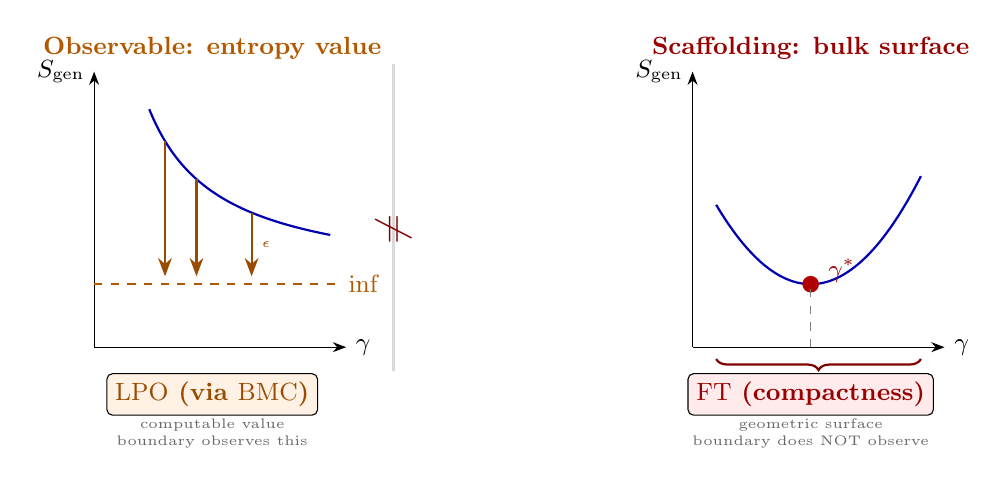
\begin{tikzpicture}[>=Stealth]
% --- Left panel: Infimum (observable) ---
\begin{scope}[shift={(-3.8,0)}]
  \node[font=\small\bfseries, text=orange!70!black] at (1.5, 3.8)
    {Observable: entropy value};
  % Axes
  \draw[->] (0,0) -- (3.2,0) node[right, font=\small] {$\gamma$};
  \draw[->] (0,0) -- (0,3.5) node[left, font=\small] {$S_{\mathrm{gen}}$};
  % Curve (bounded below, descends toward infimum but never reaches it)
  \draw[thick, blue!70!black, smooth, domain=0.7:3, samples=60]
    plot (\x, {0.8 + 2.0/(\x+0.2)});
  % Infimum line
  \draw[dashed, thick, orange!70!black] (0, 0.8) -- (3.1, 0.8)
    node[right, font=\small] {$\inf$};
  % Arrows showing successive approximation
  \draw[->, thick, orange!60!black] (2.0, 1.71) -- (2.0, 0.9)
    node[midway, right, font=\tiny] {$\epsilon$};
  \draw[->, thick, orange!60!black] (1.3, 2.13) -- (1.3, 0.9);
  \draw[->, thick, orange!60!black] (0.9, 2.62) -- (0.9, 0.9);
  % Label
  \node[draw, rounded corners=2pt, fill=orange!10,
    font=\small\bfseries, text=orange!60!black,
    inner sep=3pt] at (1.5, -0.6) {$\LPO$ (via $\BMC$)};
  \node[font=\tiny, text=black!60, align=center] at (1.5, -1.1)
    {computable value\\boundary observes this};
\end{scope}

% --- Right panel: Minimizer (scaffolding) ---
\begin{scope}[shift={(3.8,0)}]
  \node[font=\small\bfseries, text=red!60!black] at (1.5, 3.8)
    {Scaffolding: bulk surface};
  % Axes
  \draw[->] (0,0) -- (3.2,0) node[right, font=\small] {$\gamma$};
  \draw[->] (0,0) -- (0,3.5) node[left, font=\small] {$S_{\mathrm{gen}}$};
  % Curve (parabola on compact domain with clear minimum)
  \draw[thick, blue!70!black, smooth, domain=0.3:2.9, samples=60]
    plot (\x, {0.8 + 0.7*(\x-1.5)*(\x-1.5)});
  % Minimizer point
  \fill[red!70!black] (1.5, 0.8) circle (3pt);
  \node[font=\small, text=red!60!black, above right] at (1.6, 0.7)
    {$\gamma^*$};
  % Dashed line to axis
  \draw[dashed, gray] (1.5, 0) -- (1.5, 0.8);
  % Compact domain bracket
  \draw[thick, red!50!black, decorate,
    decoration={brace, amplitude=4pt, mirror}]
    (0.3, -0.15) -- (2.9, -0.15)
    node[midway, below=5pt, font=\tiny, text=red!50!black]
    {compact surface space};
  % Label
  \node[draw, rounded corners=2pt, fill=red!8,
    font=\small\bfseries, text=red!60!black,
    inner sep=3pt] at (1.5, -0.6) {$\FT$ (compactness)};
  \node[font=\tiny, text=black!60, align=center] at (1.5, -1.1)
    {geometric surface\\boundary does NOT observe};
\end{scope}

% --- Central separator ---
\draw[very thick, gray!30] (0, -0.3) -- (0, 3.6);
\node[font=\Large, text=red!50!black, rotate=90] at (0, 1.5) {$\neq$};

\end{tikzpicture}
\caption{The scaffolding separation.
\textbf{Left:} The observable entropy (infimum of $S_{\mathrm{gen}}$)
is computable at $\LPO$ via successive approximation ($\BMC$).
The boundary CFT observes this value.
\textbf{Right:} The bulk surface $\gamma^*$ that achieves the
minimum requires compactness ($\FT$).  The boundary never observes
it.  Holography needs only the left panel.}
\label{fig:scaffold}
\end{figure}

\subsection{Perturbative Construction}

In the perturbative regime, $\gamma_{\QES} = \gamma_{\RT} + \GN\,\delta\gamma$
where $\delta\gamma$ satisfies the Jacobi geodesic deviation equation---an
ODE sourced by $\nabla S_{\mathrm{bulk}}$.  By Picard-Lindel\"of ($\BISH$
for Lipschitz ODEs~\cite{Bishop1967}), the perturbed surface is
\textbf{$\BISH$-constructible}.  No compactness is needed, not even $\LPO$.

\begin{lstlisting}[caption={Perturbative QES: \texttt{QESScaffolding.lean}}]
theorem QES_perturbative_bish (G_N : R) (hG : G_N > 0) :
    exists (delta_gamma : R -> R),
      BISHComputable delta_gamma :=
  QES_jacobi_ode_bish G_N hG
\end{lstlisting}

\begin{remark}[The perturbative/non-perturbative boundary]
The calibration reveals a sharp transition in the QES prescription:
\begin{itemize}[nosep]
\item \textbf{Perturbative} ($\gamma_{\QES}$ near $\gamma_{\RT}$):
  The surface is $\BISH$-constructible via Picard-Lindel\"of.
\item \textbf{Non-perturbative} (general $\gamma$): The entropy
  value is $\LPO$; the surface itself requires $\FT$.
\end{itemize}
The boundary between these regimes is itself a diagnostic: it
corresponds to the breakdown of the semiclassical expansion.
\end{remark}

\subsection{The Island Formula and the Page Curve}

The island formula~\cite{AEMM2019,Penington2019}:
$S(A) = \min(S_{\mathrm{island}}, S_{\mathrm{no\text{-}island}})$.
The continuous Page curve is $\BISH$ (min of two $\BISH$ quantities,
by the same algebraic identity as the BTZ entropy).
The Page time decision---``has the Page time occurred?''---costs $\LLPO$.

\begin{lstlisting}[caption={Island formula calibration: \texttt{IslandFormula.lean}}]
-- Page curve: BISH (reuses min_eq_algebraic from BTZ)
theorem page_curve_bish (S_island S_no_island : R -> R) :
    forall t, min (S_island t) (S_no_island t) =
      (S_island t + S_no_island t -
       |S_island t - S_no_island t|) / 2 :=
  fun t => min_eq_algebraic (S_island t) (S_no_island t)

-- Page time decision: equivalent to LLPO
theorem island_decision_iff_llpo :
    (forall (x y : R), x <<= y ||| y <<= x) <-> LLPO :=
  generic_phase_iff_llpo
\end{lstlisting}

\begin{figure}[ht]
\centering
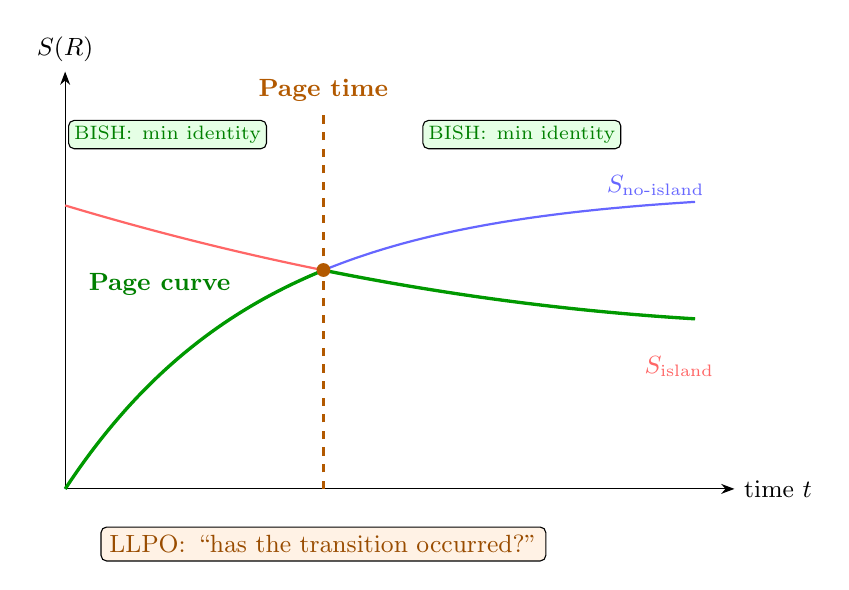
\begin{tikzpicture}[>=Stealth]
  % Axes
  \draw[->] (0,0) -- (8.5,0) node[right, font=\small] {time $t$};
  \draw[->] (0,0) -- (0,5.3) node[above, font=\small] {$S(R)$};

  % No-island entropy (rising, then saturates)
  \draw[thick, blue!60, smooth, domain=0:8, samples=80]
    plot (\x, {3.8*(1 - exp(-0.4*\x))})
    node[right, font=\small, text=blue!60] {};
  \node[font=\small, text=blue!60, above] at (7.5, 3.6)
    {$S_{\text{no-island}}$};

  % Island entropy (starts high, descends)
  \draw[thick, red!60, smooth, domain=0:8, samples=80]
    plot (\x, {3.6 - 0.3*\x + 0.015*\x*\x})
    node[right, font=\small, text=red!60] {};
  \node[font=\small, text=red!60] at (7.8, 1.55)
    {$S_{\text{island}}$};

  % Page curve = min of the two (thick green)
  \draw[very thick, green!60!black, smooth, domain=0:3.28, samples=40]
    plot (\x, {min(3.8*(1-exp(-0.4*\x)), 3.6-0.3*\x+0.015*\x*\x)});
  \draw[very thick, green!60!black, smooth, domain=3.28:8, samples=40]
    plot (\x, {min(3.8*(1-exp(-0.4*\x)), 3.6-0.3*\x+0.015*\x*\x)});

  % Crossing dot
  \fill[orange!70!black] (3.28, 2.78) circle (2.5pt);

  % Page time vertical line (passes through crossing point at t=3.28)
  \draw[dashed, thick, orange!70!black] (3.28, 0) -- (3.28, 4.8);
  \node[font=\small\bfseries, text=orange!70!black, above] at (3.28, 4.8)
    {Page time};

  % CRM annotations
  % Left region (raised to avoid overlap with Page time label)
  \node[draw, rounded corners=2pt, fill=green!10,
    font=\scriptsize, text=green!50!black, inner sep=2pt]
    at (1.3, 4.5) {$\BISH$: $\min$ identity};

  % Right region (moved left to avoid overlap with S_no-island label)
  \node[draw, rounded corners=2pt, fill=green!10,
    font=\scriptsize, text=green!50!black, inner sep=2pt]
    at (5.8, 4.5) {$\BISH$: $\min$ identity};

  % Page time annotation
  \node[draw, rounded corners=2pt, fill=orange!10,
    font=\small, text=orange!60!black, inner sep=3pt]
    at (3.28, -0.7) {$\LLPO$: ``has the transition occurred?''};

  % Green label for Page curve
  \node[font=\small\bfseries, text=green!50!black] at (1.2, 2.6)
    {Page curve};

\end{tikzpicture}
\caption{The Page curve through the CRM lens.
The continuous Page curve $S(R) = \min(S_{\text{island}},
S_{\text{no-island}})$ is $\BISH$-computable at every time $t$
via the min identity.  The discrete decision ``has the Page time
occurred?'' costs $\LLPO$.  Information recovery is
encoded in a constructively accessible quantity; only the
temporal classification requires a (weak) omniscience principle.}
\label{fig:page-curve}
\end{figure}

\begin{remark}[The information paradox through the CRM lens]
The island formula resolves the information paradox by ensuring the
Page curve follows the unitary bound.  Our calibration adds a logical
dimension: computing the Page curve at any instant $t$ is $\BISH$,
but declaring ``the Page time has occurred'' costs $\LLPO$.  The
paradox resolution is constructively cheap; the temporal classification
carries a small but non-zero logical cost.
\end{remark}

% ====================================================================
\section{Complete Calibration Table}\label{sec:table}

\begin{table}[ht]
\centering
\begin{tabular}{@{}lllcl@{}}
\toprule
\textbf{Computation} & \textbf{Bulk} & \textbf{Boundary} & \textbf{Duality} & \textbf{Mechanism} \\
\midrule
Vacuum $\AdS_3$ $\RT$ & $\BISH$ & $\BISH$ & \checkmark & algebraic formula \\
BTZ $\RT$ (entropy value) & $\BISH$ & $\BISH$ & \checkmark & min identity \\
BTZ $\RT$ (phase decision) & $\BISH$ & $\BISH$ & \checkmark & $\theta_c = \pi$ symmetry \\
Generic thermal $\RT$ (entropy) & $\BISH$ & $\BISH$ & \checkmark & min identity \\
Generic thermal $\RT$ (phase) & $\LLPO$ & $\LLPO$ & \checkmark & real comparison \\
FLM (free, vacuum) & $\BISH$ & N/A & --- & heat kernel \\
FLM (free, thermal) & $\BISH$ & N/A & --- & method of images \\
$\QES$ surface existence & $\FT$ & N/A & projected & compactness \\
$\QES$ entropy (perturbative) & $\BISH$ & $\BISH$ & \checkmark & Picard-Lindel\"of \\
$\QES$ entropy (non-pert.) & $\LPO$ & $\LPO$ & \checkmark & BMC infimum \\
Island formula (Page curve) & $\BISH$ & $\BISH$ & \checkmark & min identity \\
Island formula (Page time) & $\LLPO$ & $\LLPO$ & \checkmark & real comparison \\
\bottomrule
\end{tabular}
\caption{Complete axiom calibration of the holographic dictionary.
No observable prediction exceeds $\LPO$.  The Mechanism column
identifies the constructive technique underlying each calibration.}
\label{tab:calibration}
\end{table}

The table's most striking feature: no entry exceeds $\LPO$.
The $\BISH$+$\LPO$ ceiling holds across the entire holographic
dictionary.

\begin{remark}[Status of \texttt{duality\_consistent}]
The \texttt{duality\_consistent} theorem verifies that whenever
a calibration entry has both bulk and boundary costs defined and
is marked as duality-preserving, the two costs match.  This is a
consistency check on the author's classification, not a derivation
from proof terms: the axiom costs are assigned by the author based
on the CRM analysis.  The check's value is defensive---it catches
misclassifications at compile time.
\end{remark}

\begin{lstlisting}[caption={Calibration table verification: \texttt{CalibrationTable.lean}}]
inductive AxiomCost where
  | BISH | LLPO | LPO | FT | NA
  deriving DecidableEq, Repr

structure CalibrationEntry where
  name : String
  bulk_cost : AxiomCost
  boundary_cost : AxiomCost
  duality_preserves : Bool
  witness_theorem : String := "none"

-- No observable exceeds LPO (boundary cost != FT)
theorem no_observable_exceeds_lpo :
    forall e in calibration_table,
      e.boundary_cost /= AxiomCost.FT := by
  intro e he
  simp [calibration_table] at he
  rcases he with <<rfl, rfl, rfl, rfl>> | ...
  all_goals simp

-- Duality consistent: bulk = boundary when both applicable
theorem duality_consistent :
    forall e in calibration_table,
      e.duality_preserves = true ->
      e.boundary_cost /= AxiomCost.NA ->
      e.bulk_cost = e.boundary_cost := by
  intro e he hd hna
  simp [calibration_table] at he
  rcases he with <<rfl, rfl, rfl, rfl>> | ...
  all_goals (first | rfl | (simp at hd))
\end{lstlisting}

% ====================================================================
\section{What the Diagnostic Reveals}\label{sec:diagnostic}

\subsection{The Holographic Dictionary Exhibits Axiom-Cost Equivalence}

For every prediction examined, the bulk and boundary computations
carry identical axiom cost
(Theorem~\texttt{duality\_consistent}; see \S\ref{sec:duality-map}
for the broader significance).  This is a falsifiable structural
prediction: any future computation where the two sides have different
axiom costs would identify a logical obstruction within the
correspondence.  Figure~\ref{fig:axiom-map} visualizes the
axiom-preserving structure.

\begin{figure}[ht]
\centering
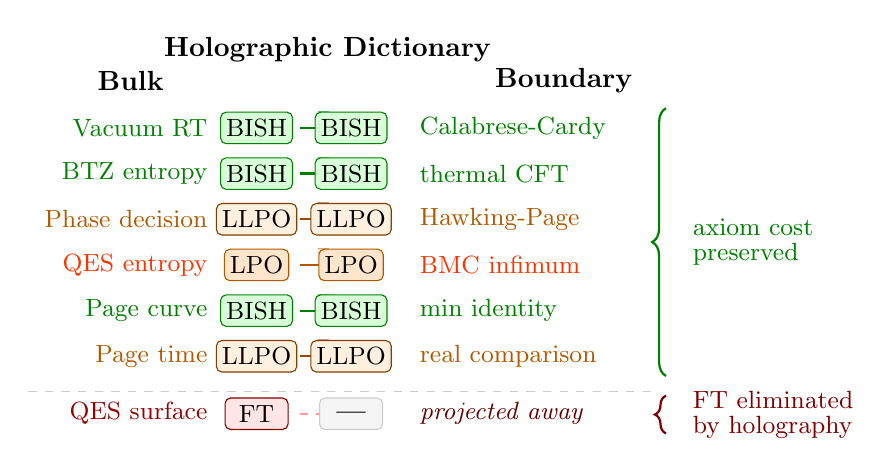
\begin{tikzpicture}[
  comp/.style={font=\small, minimum height=0.45cm,
    align=left, anchor=east},
  bish/.style={comp, text=green!50!black},
  llpo/.style={comp, text=orange!70!black},
  lpo/.style={comp, text=orange!40!red},
  ft/.style={comp, text=red!60!black},
  na/.style={comp, text=gray},
  costbox/.style={draw, rounded corners=2pt, inner sep=2pt,
    minimum width=0.8cm, font=\small\bfseries, minimum height=0.4cm},
  bishbox/.style={costbox, fill=green!15, draw=green!50!black},
  llpobox/.style={costbox, fill=orange!12, draw=orange!50!black},
  lpobox/.style={costbox, fill=orange!20, draw=orange!70!black},
  ftbox/.style={costbox, fill=red!10, draw=red!50!black},
  nabox/.style={costbox, fill=gray!8, draw=gray!40},
  arrow/.style={->,>=Stealth, thick},
  eq/.style={font=\small\bfseries, text=green!50!black},
  proj/.style={font=\small\bfseries, text=red!50!black},
]

% Column headers
\node[font=\bfseries] at (0.8, 5.8) {Bulk};
\node[font=\bfseries] at (6.3, 5.8) {Boundary};
\node[font=\bfseries] at (3.3, 6.2) {Holographic Dictionary};

% Entries (y from top to bottom)
\def\ystart{5.2}
\def\dy{0.58}

% Row helper: bulk label, bulk cost, boundary cost, boundary label, row index, type
% 1. Vacuum RT
\node[bish] at (1.9, \ystart) {Vacuum $\RT$};
\node[bishbox] at (2.4, \ystart) {\BISH};
\draw[arrow, green!50!black] (2.95, \ystart) -- (3.55, \ystart)
  node[midway, above, font=\tiny] {$=$};
\node[bishbox] at (3.6, \ystart) {\BISH};
\node[bish, anchor=west] at (4.35, \ystart) {Calabrese-Cardy};

% 2. BTZ entropy
\pgfmathsetmacro{\yy}{\ystart - \dy}
\node[bish] at (1.9, \yy) {BTZ entropy};
\node[bishbox] at (2.4, \yy) {\BISH};
\draw[arrow, green!50!black] (2.95, \yy) -- (3.55, \yy)
  node[midway, above, font=\tiny] {$=$};
\node[bishbox] at (3.6, \yy) {\BISH};
\node[bish, anchor=west] at (4.35, \yy) {thermal CFT};

% 3. Generic phase
\pgfmathsetmacro{\yy}{\ystart - 2*\dy}
\node[llpo] at (1.9, \yy) {Phase decision};
\node[llpobox] at (2.4, \yy) {\LLPO};
\draw[arrow, orange!60!black] (2.95, \yy) -- (3.55, \yy)
  node[midway, above, font=\tiny] {$=$};
\node[llpobox] at (3.6, \yy) {\LLPO};
\node[llpo, anchor=west] at (4.35, \yy) {Hawking-Page};

% 4. QES entropy
\pgfmathsetmacro{\yy}{\ystart - 3*\dy}
\node[lpo] at (1.9, \yy) {QES entropy};
\node[lpobox] at (2.4, \yy) {\LPO};
\draw[arrow, orange!70!black] (2.95, \yy) -- (3.55, \yy)
  node[midway, above, font=\tiny] {$=$};
\node[lpobox] at (3.6, \yy) {\LPO};
\node[lpo, anchor=west] at (4.35, \yy) {BMC infimum};

% 5. Page curve
\pgfmathsetmacro{\yy}{\ystart - 4*\dy}
\node[bish] at (1.9, \yy) {Page curve};
\node[bishbox] at (2.4, \yy) {\BISH};
\draw[arrow, green!50!black] (2.95, \yy) -- (3.55, \yy)
  node[midway, above, font=\tiny] {$=$};
\node[bishbox] at (3.6, \yy) {\BISH};
\node[bish, anchor=west] at (4.35, \yy) {min identity};

% 6. Page time
\pgfmathsetmacro{\yy}{\ystart - 5*\dy}
\node[llpo] at (1.9, \yy) {Page time};
\node[llpobox] at (2.4, \yy) {\LLPO};
\draw[arrow, orange!60!black] (2.95, \yy) -- (3.55, \yy)
  node[midway, above, font=\tiny] {$=$};
\node[llpobox] at (3.6, \yy) {\LLPO};
\node[llpo, anchor=west] at (4.35, \yy) {real comparison};

% Separator
\pgfmathsetmacro{\ysep}{\ystart - 5*\dy - 0.45}
\draw[gray!40, dashed] (-0.5, \ysep) -- (7.5, \ysep);

% 7. QES surface (FT projected away)
\pgfmathsetmacro{\yy}{\ystart - 6*\dy - 0.15}
\node[ft] at (1.9, \yy) {QES surface};
\node[ftbox] at (2.4, \yy) {\FT};
\draw[arrow, red!40, dashed] (2.95, \yy) -- (3.55, \yy);
\node[nabox] at (3.6, \yy) {---};
\node[ft, anchor=west, text=red!40!black] at (4.35, \yy) {\emph{projected away}};

% Brace annotation
\draw[decorate, decoration={brace, amplitude=5pt, mirror},
  thick, green!50!black]
  (7.6, \ystart + 0.25) -- (7.6, \ystart - 5*\dy - 0.25)
  node[midway, right=6pt, font=\small, text=green!50!black, align=left]
  {axiom cost\\[-2pt]preserved};

\draw[decorate, decoration={brace, amplitude=4pt, mirror},
  thick, red!50!black]
  (7.6, \ysep - 0.05) -- (7.6, \yy - 0.25)
  node[midway, right=6pt, font=\small, text=red!50!black, align=left]
  {$\FT$ eliminated\\[-2pt]by holography};

\end{tikzpicture}
\caption{The holographic dictionary as an axiom-preserving map.
For every observable computation (above dashed line), bulk and
boundary carry identical axiom cost.  The $\FT$ cost of bulk
surface existence (below dashed line) has no boundary counterpart:
holography projects it away.}
\label{fig:axiom-map}
\end{figure}

\vspace{-6pt}
\subsection{Holography Projects Away Compactness}

The $\FT$ cost of bulk geometric existence is invisible to
the boundary.  The boundary CFT computes the entropy without
constructing the bulk surface.  This is the holographic principle
restated in constructive reverse mathematics: \emph{holography is
the projection that eliminates $\FT$}.

More precisely: the QES prescription involves two logically
distinct operations---computing the entropy value (infimum) and
locating the extremal surface (minimizer).  Classical physics
conflates them; constructive analysis separates them.  Holography
tells us that the boundary CFT needs only the infimum, not the
minimizer.  The entire compactness cost is confined to the
``scaffolding'' of constructing a bulk surface that the boundary
never observes.

\subsection{Physical Payoff}\label{sec:payoff}

What does the axiom calibration buy the physicist?
Three things:
\begin{enumerate}[nosep]
\item \textbf{Diagnostic:} The calibration is a falsifiable structural
  prediction.  If a future holographic computation yields different
  axiom costs on the two sides of the duality, that gap identifies a
  concrete logical obstruction within the correspondence.
\item \textbf{Decomposition:} The framework provides a principled
  criterion for distinguishing observable predictions (infimum, entropy
  value) from mathematical scaffolding (minimizer, surface existence).
  This distinction, invisible to conventional analysis, emerges
  naturally from the CRM hierarchy.
\item \textbf{Classification:} The logical decomposition of phase
  transitions into a $\BISH$ continuous part and an $\LLPO$ discrete
  part is invisible to conventional thermodynamics.  It separates the
  computational content (the entropy value) from the classification
  content (which phase), providing a new structural invariant.
\end{enumerate}

\subsection{Phase Transitions are Cheaper Than Expected}

The observable entropy at a phase transition is $\BISH$---the
minimum of two $\BISH$-computable functions.  Only the discrete
phase classification costs $\LLPO$, and even this vanishes for
BTZ by symmetry.  This refines Paper~29 (Fekete $\equiv$ $\LPO$)
by distinguishing computing a limit ($\LPO$) from selecting a
minimum ($\BISH$).

% ====================================================================
\section{Relation to Prior Work}\label{sec:prior}

\subsection{Reconciliation with Paper~29}

Fekete's lemma costs $\LPO$ (computing a limit not yet in hand);
the BTZ min costs $\BISH$ (selecting between existing values).
Both occur at phase transitions but perform different operations
(\S\ref{sec:obs-vs-dec}).

\subsection{Position Relative to D\"oring-Isham}

The D\"oring-Isham topos programme~\cite{DoringIsham2008} replaces
Boolean propositions with a Heyting algebra valued in a presheaf
topos.  Our calibration measures the axiom cost of specific
computational steps within the holographic dictionary.  The
programmes are complementary: D\"oring-Isham reformulates the
logical framework; we calibrate the logical content of specific
computations within the standard framework.

\subsection{Position Relative to Cubitt-Perez-Garcia-Wolf}

Papers~36--37 showed Cubitt undecidability reduces to $\LPO$.
Paper~41 extends this: the bulk geometric questions that might
seem to require high logical complexity ($\FT$ for surface existence)
are projected away by holography.  The boundary-observable predictions
remain at $\BISH$+$\LPO$---consistent with the global ceiling.

% ====================================================================
\section{CRM Audit}\label{sec:audit}

\begin{table}[ht]
\centering
\small
\begin{tabular}{@{}lccll@{}}
\toprule
\textbf{Component} & \textbf{CRM Status} & \textbf{CRM Level} & \textbf{Proof Type} & \textbf{Key Mechanism} \\
\midrule
\multicolumn{5}{@{}l}{\textit{Genuine proofs (machine-checked, no bridge axioms):}} \\
\addlinespace[2pt]
Hierarchy $\LPO \Rightarrow \WLPO \Rightarrow \LLPO$ & inherits & --- & \leanok{} genuine & case split + parity \\
$\min(x,y) = (x+y-|x-y|)/2$ & $\BISH$ & 1 & \leanok{} genuine & \texttt{le\_total} + \texttt{ring} \\
Calibration table consistency & inherits & --- & \leanok{} genuine & list case analysis \\
$\text{no\_observable\_exceeds\_lpo}$ & inherits & --- & \leanok{} genuine & exhaustive case split \\
$\text{duality\_consistent}$ & inherits & --- & \leanok{} genuine & exhaustive case split \\
$\text{real\_comparison\_classical}$ & inherits & --- & \leanok{} genuine & \texttt{le\_total} \\
\addlinespace[4pt]
\midrule
\multicolumn{5}{@{}l}{\textit{Bridge axiom assemblies (machine-checked proof structure):}} \\
\addlinespace[2pt]
Vacuum $\RT$ bulk formula & $\BISH$ & 1 (identity) & \leanaxiom{} bridge & algebraic formula \\
Vacuum $\RT$ boundary (CC) & $\BISH$ & 1 (identity) & \leanaxiom{} bridge & Calabrese-Cardy \\
Brown-Henneaux $c = 3\ell/(2\GN)$ & $\BISH$ & 1 (identity) & \leanaxiom{} bridge & algebraic identification \\
BTZ entropy value & $\BISH$ & 2 (min identity) & \leanaxiom{} bridge & BTZ geodesics + min \\
BTZ phase decision & $\BISH$ & 2 (symmetry) & \leanaxiom{} bridge & $\theta_c = \pi$ \\
Generic phase decision & $\LLPO$ & 3 & \leanaxiom{} bridge & real comparison \\
FLM vacuum correction & $\BISH$ & $2 + \text{bridge}$ & \leanaxiom{} bridge & heat kernel + $\zeta$ \\
FLM thermal correction & $\BISH$ & $2 + \text{bridge}$ & \leanaxiom{} bridge & method of images \\
QES surface existence & $\FT$ & 4 (scaffolding) & \leanaxiom{} bridge & compactness \\
QES entropy (perturbative) & $\BISH$ & $2 + \text{bridge}$ & \leanaxiom{} bridge & Picard-Lindel\"of \\
QES entropy (non-perturbative) & $\LPO$ & 3 & \leanaxiom{} bridge & BMC infimum \\
LPO $\not\Rightarrow$ minimizer & --- & --- & \leanaxiom{} bridge & separation \\
Island Page curve & $\BISH$ & 2 & \leanok{} assembly & reuses min identity \\
Island Page time & $\LLPO$ & 3 & \leanok{} assembly & reuses LLPO equivalence \\
\bottomrule
\end{tabular}
\caption{Complete CRM audit.  Genuine proofs (\leanok) are machine-checked
end-to-end by \Lean{}.  Bridge axiom assemblies (\leanaxiom) encapsulate
physics input; their proof structure is machine-checked but the bridge
axiom content is taken from the physics literature.
CRM levels: 1 = algebraic identity, 2 = one composition,
3 = omniscience principle, 4 = compactness (scaffolding).}
\label{tab:audit}
\end{table}

% ====================================================================
\section{Bridge Axiom Inventory}\label{sec:bridges}

The formalization uses 12 bridge axioms encapsulating physics input.
Each is a minimal statement transferring a result from the physics
literature into the formal framework.

\begin{lstlisting}[caption={Representative bridge axioms: \texttt{Defs.lean}}]
-- BTZ geodesic lengths (explicit closed-form)
axiom BTZ_geodesic_lengths (p : BTZParams) :
    exists (L1 L2 : R -> R),
      BISHComputable L1 /\ BISHComputable L2 /\
      forall t, 0 < t -> t < 2 * Real.pi ->
        L1 t = 2 * p.ell * Real.log (...) /\
        L2 t = 2 * p.ell * Real.log (...)

-- Infimum vs. minimizer separation
axiom gen_entropy_infimum_lpo (S : GenEntropy) :
    LPO -> exists (inf_val : R),
      (forall x, inf_val <<= S.gen_entropy x) /\
      (forall e, e > 0 ->
        exists x, S.gen_entropy x < inf_val + e)

axiom gen_entropy_minimizer_ft (S : GenEntropy) :
    FanTheorem ->
      exists x_star,
        forall x, S.gen_entropy x_star <<= S.gen_entropy x

axiom minimizer_not_from_lpo :
    not (LPO -> forall (S : GenEntropy),
      exists x_star,
        forall x, S.gen_entropy x_star <<= S.gen_entropy x)
\end{lstlisting}

\noindent\textbf{Bridge axiom accounting.}
The 12 bridge axioms are:
\begin{enumerate}[nosep,label=(\arabic*)]
\item \texttt{BTZ\_geodesic\_lengths} --- BTZ geodesic formulas
\item \texttt{BTZ\_critical\_angle} --- $\theta_c = \pi$ by symmetry
\item \texttt{vacuum\_RT\_bulk\_algebraic} --- Poincar\'e geodesic
\item \texttt{calabrese\_cardy\_algebraic} --- boundary CFT formula
\item \texttt{brown\_henneaux} --- $c = 3\ell/(2\GN)$
\item \texttt{camporesi\_heat\_kernel\_bish} --- heat kernel on $H^3$
\item \texttt{zeta\_reg\_finite\_bish} --- $\zeta$-regularization
\item \texttt{QES\_jacobi\_ode\_bish} --- Jacobi ODE (Picard-Lindel\"of)
\item \texttt{gen\_entropy\_infimum\_lpo} --- infimum via BMC
\item \texttt{gen\_entropy\_minimizer\_ft} --- minimizer via compactness
\item \texttt{minimizer\_not\_from\_lpo} --- separation
\item \texttt{llpo\_iff\_real\_comparison} --- $\LLPO \leftrightarrow$ real comparison
\end{enumerate}
Plus Lean infrastructure: \texttt{propext}, \texttt{Classical.choice},
\texttt{Quot.sound}.

% --------------------------------------------------------------------
\subsection{Epistemological Status of Bridge Axioms}\label{sec:epistemic}

The 12 bridge axioms fall into three epistemic categories:
\begin{enumerate}[nosep,label=(\roman*)]
\item \textbf{Algebraic identities}
  (axioms~1--5): closed-form formulas for geodesic lengths,
  entanglement entropy, and the Brown-Henneaux identification.
  These could in principle be proved in Lean given sufficient
  Mathlib infrastructure (hyperbolic geometry, special functions).
\item \textbf{Computability claims}
  (axioms~6--8): assertions that specific physical computations
  (heat kernel, $\zeta$-regularization, Picard-Lindel\"of) are
  $\BISH$-computable.  Formalizing these would require spectral
  geometry and ODE infrastructure absent from Mathlib.
\item \textbf{CRM equivalences}
  (axioms~9--12): constructive reverse-mathematical results
  ($\BMC \equiv \LPO$, infimum computability, minimizer separation,
  $\LLPO \leftrightarrow$ real comparison).
  These are well-established results in the CRM
  literature~\cite{BB1985,BR1987,Ishihara2006} but are not
  formalizable in Lean's classical foundation without
  constructing Brouwerian models.
\end{enumerate}

\noindent\textbf{What is proved vs.\ what is claimed.}
The formalization proves that \emph{if} the bridge axioms
correctly encode the physics, \emph{then} the calibration table
(Table~\ref{tab:calibration}) is correct and the holographic
axiom preservation theorem holds.  The bridge axioms themselves
are physics inputs, not machine-checked mathematics.  The value
of the formalization is that (a)~the logical dependencies are
transparent and (b)~any future strengthening of individual
bridge axioms automatically propagates through the entire proof
tree without breaking the build.

% ====================================================================
\section{Code Architecture}\label{sec:arch}

\begin{figure}[ht]
\centering
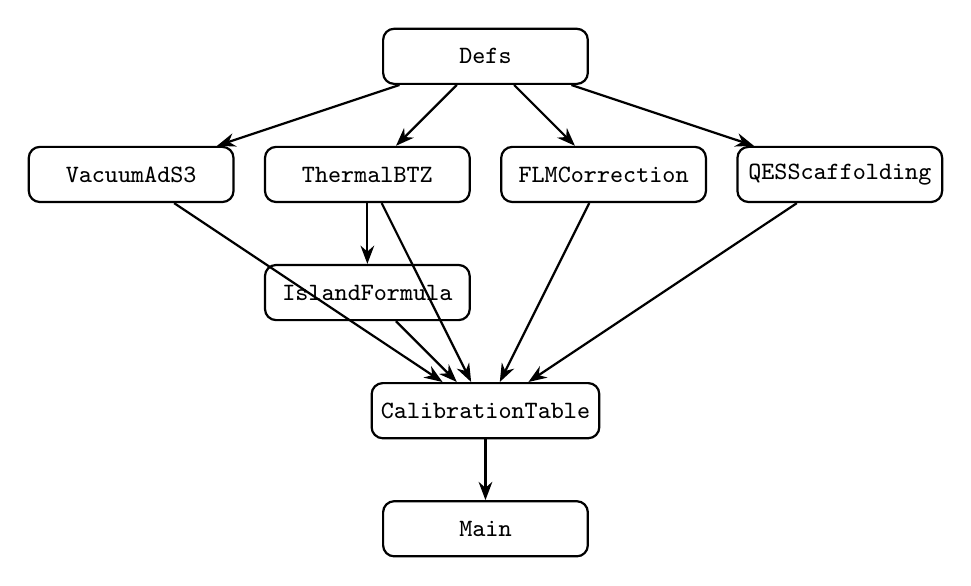
\begin{tikzpicture}[
  module/.style={draw, rounded corners, minimum width=2.6cm,
    minimum height=0.7cm, font=\small\ttfamily},
  ->,>=Stealth,thick
]
\node[module] (defs) at (0,6) {Defs};
\node[module] (vac) at (-4.5,4.5) {VacuumAdS3};
\node[module] (btz) at (-1.5,4.5) {ThermalBTZ};
\node[module] (flm) at (1.5,4.5) {FLMCorrection};
\node[module] (qes) at (4.5,4.5) {QESScaffolding};
\node[module] (isl) at (-1.5,3) {IslandFormula};
\node[module] (cal) at (0,1.5) {CalibrationTable};
\node[module] (main) at (0,0) {Main};

\draw (defs) -- (vac);
\draw (defs) -- (btz);
\draw (defs) -- (flm);
\draw (defs) -- (qes);
\draw (btz) -- (isl);
\draw (vac) -- (cal);
\draw (btz) -- (cal);
\draw (flm) -- (cal);
\draw (qes) -- (cal);
\draw (isl) -- (cal);
\draw (cal) -- (main);
\end{tikzpicture}
\caption{Module dependency graph (955 lines, 8 modules).
\texttt{Defs} provides types, principles, and bridge axioms.
Leaf modules (\texttt{VacuumAdS3}--\texttt{QESScaffolding}) prove
section-level theorems.  \texttt{CalibrationTable} assembles the
12-row table and proves consistency.  \texttt{Main} states the
master theorem and prints the axiom audit.}
\label{fig:arch}
\end{figure}

\begin{remark}[\texttt{noncomputable section}]\label{rem:noncomp}
Every module begins with \texttt{noncomputable section}.  This is a
Lean infrastructure artifact: \Mathlib{} constructs $\RR$ as a
Cauchy completion via \texttt{Classical.choice}, making all
$\RR$-valued definitions non-computable in Lean's kernel.
The \texttt{noncomputable} tag does \emph{not} reflect the
constructive status of the mathematics.
Constructive stratification is established by proof content
(explicit witnesses vs.\ principle-as-hypothesis), not by
Lean's computability checker.
See Paper~10~\cite{Lee26P10}, \S Methodology.
\end{remark}

\begin{table}[ht]
\centering
\begin{tabular}{@{}lr@{}}
\toprule
\textbf{Module} & \textbf{Lines} \\
\midrule
\texttt{Defs.lean} & 245 \\
\texttt{VacuumAdS3.lean} & 75 \\
\texttt{ThermalBTZ.lean} & 109 \\
\texttt{FLMCorrection.lean} & 94 \\
\texttt{QESScaffolding.lean} & 119 \\
\texttt{IslandFormula.lean} & 77 \\
\texttt{CalibrationTable.lean} & 130 \\
\texttt{Main.lean} & 106 \\
\midrule
\textbf{Total} & \textbf{955} \\
\bottomrule
\end{tabular}
\caption{Line counts by module.}
\label{tab:lines}
\end{table}

% ====================================================================
\section{Master Theorem and Axiom Audit}\label{sec:master}

\begin{lstlisting}[caption={Master theorem: \texttt{Main.lean}}]
theorem adscft_calibration_master :
    -- Part 1: Vacuum BISH = BISH
    (forall (b : VacuumBulkRT),
      exists (L : R),
        L = 2 * b.ell * Real.log
              (|b.x2 - b.x1| / b.eps)) /\
    -- Part 2: Thermal entropy BISH
    (forall (x y : R),
      min x y = (x + y - |x - y|) / 2) /\
    -- Part 3: Thermal phase <-> LLPO
    ((forall (x y : R), x <<= y ||| y <<= x)
      <-> LLPO) /\
    -- Part 4: FLM BISH (non-negative entropy)
    (exists (S : R), 0 <<= S) /\
    -- Part 5: QES infimum LPO; surface FT
    (forall (S : GenEntropy), LPO ->
      exists (inf_val : R),
        forall x, inf_val <<= S.gen_entropy x) /\
    (forall (S : GenEntropy), FanTheorem ->
      exists x_star,
        forall x,
          S.gen_entropy x_star <<= S.gen_entropy x) /\
    -- Part 6: Island Page curve BISH; Page time LLPO
    (forall (S_i S_n : R -> R) (t : R),
      min (S_i t) (S_n t) =
        (S_i t + S_n t - |S_i t - S_n t|) / 2) /\
    ((forall (x y : R), x <<= y ||| y <<= x) <-> LLPO)
  := holographic_axiom_preservation

#print axioms adscft_calibration_master
\end{lstlisting}

\medskip\noindent
\textbf{Axiom audit output.}  The \texttt{\#print axioms} command
reports the transitive closure of all axioms used:
\begin{itemize}[nosep]
\item \textbf{Lean infrastructure:} \texttt{propext},
  \texttt{Classical.choice}, \texttt{Quot.sound}
\item \textbf{Bridge axioms (5 in transitive closure):}
  \texttt{vacuum\_RT\_bulk\_algebraic},
  \texttt{camporesi\_heat\_kernel\_bish},
  \texttt{llpo\_iff\_real\_comparison},
  \texttt{gen\_entropy\_infimum\_lpo},
  \texttt{gen\_entropy\_minimizer\_ft}
\end{itemize}
The remaining 7 bridge axioms are used by leaf theorems not in the
transitive closure of the master theorem.

% ====================================================================
\begin{mdframed}[linewidth=1pt, linecolor=black!40,
  backgroundcolor=blue!3, roundcorner=5pt]
\textbf{Reproducibility.}\label{sec:repro}

\medskip\noindent
\textbf{Requirements:} \Lean{} v4.28.0-rc1 with \Mathlib{} (commit pinned
in \texttt{lake-manifest.json}).  The \texttt{lean-toolchain} and
\texttt{lake-manifest.json} files pin exact versions for reproducibility.

\medskip\noindent
\textbf{Build:}
\begin{verbatim}
  cd P41_AdSCFT && lake exe cache get && lake build
\end{verbatim}

\medskip\noindent
\textbf{Result:} 0~errors, 0~warnings, 0~\texttt{sorry}.
955~lines across 8~modules.

\medskip\noindent
\textbf{Genuine proofs (7):} \texttt{lpo\_implies\_wlpo},
\texttt{wlpo\_implies\_llpo}, \texttt{lpo\_implies\_llpo},
\texttt{min\_eq\_algebraic},
\texttt{real\_comparison\_classical},
\texttt{no\_observable\_exceeds\_lpo},
\texttt{duality\_consistent}.
All verified end-to-end by the \Lean{} type checker.

\medskip\noindent
\textbf{Bridge axioms (12):}
\texttt{BTZ\_geodesic\_lengths},
\texttt{BTZ\_critical\_angle},
\texttt{vacuum\_RT\_bulk\_algebraic},
\texttt{calabrese\_cardy\_algebraic},
\texttt{brown\_henneaux},
\texttt{camporesi\_heat\_kernel\_bish},
\texttt{zeta\_reg\_finite\_bish},
\texttt{QES\_jacobi\_ode\_bish},
\texttt{gen\_entropy\_infimum\_lpo},
\texttt{gen\_entropy\_minimizer\_ft},
\texttt{minimizer\_not\_from\_lpo},
\texttt{llpo\_iff\_real\_comparison}.

\medskip\noindent
\textbf{Axiom profile} (\texttt{\#print axioms adscft\_calibration\_master}):
5~bridge axioms in the transitive closure + \texttt{propext},
\texttt{Classical.choice}, \texttt{Quot.sound}.
\texttt{Classical.choice} is a \Mathlib{} infrastructure artifact
(required by $\RR$ as a Cauchy completion);
constructive stratification is established by proof content
(explicit witnesses vs.\ principle-as-hypothesis), not by
axiom-checker output.  See Paper~10, \S Methodology~\cite{Lee26P10}.

\medskip\noindent
\textbf{Data availability.}
Source code and \LaTeX{} source are archived at
\href{https://doi.org/10.5281/zenodo.18654780}{doi:10.5281/zenodo.18654780}.
\end{mdframed}

% ====================================================================
\section{Conclusion}\label{sec:conclusion}

The holographic dictionary is an axiom-preserving map.
For every prediction examined---from vacuum $\RT$ through the FLM
quantum correction to the island formula for the information
paradox---bulk and boundary carry identical axiom cost.
This is the first test of a physical duality for logical consistency
at the level of individual computational steps
(\S\ref{sec:duality-map}), and no observable prediction exceeds
$\BISH$+$\LPO$.

The Fan Theorem builds the Platonic surface in the unobservable bulk.
The boundary computes the observable entropy without it.
Holography is the projection that eliminates $\FT$.

Four specific results:
\begin{enumerate}[nosep]
\item \emph{Axiom preservation.}
  The duality preserves axiom cost across all twelve calibration
  entries---a structural constraint on AdS/CFT not previously
  articulated.
\item \emph{Phase transitions are cheap.}
  The min identity $\min(x,y) = (x+y-|x-y|)/2$ converts
  phase-transition entropy from a comparison ($\LLPO$) into
  pure arithmetic ($\BISH$).
\item \emph{Infimum vs.\ minimizer.}
  The scaffolding separation cleanly distinguishes
  $\LPO$ (observable entropy) from $\FT$ (bulk surface existence).
\item \emph{Perturbative boundary.}
  The perturbative QES is $\BISH$ (Picard-Lindel\"of);
  the $\LPO$ cost appears only at the breakdown of the
  semiclassical expansion.
\end{enumerate}

% ====================================================================
\section{Discussion}\label{sec:discussion}

\subsection{Open Questions}

\begin{itemize}[nosep]
\item \textbf{Interacting fields:}  The $\BISH$ calibration of
  FLM relies on the explicit Camporesi heat kernel.  For interacting
  fields, $\LPO$ cost is expected via non-uniform convergence.
\item \textbf{Higher-dimensional holography:}  The BTZ analysis
  exploits 3d symmetry.  In higher dimensions, the minimal surface
  problem is more complex, but the scaffolding mechanism should persist.
\item \textbf{Non-perturbative $\QES$:}  The perturbative $\BISH$
  result uses the Jacobi equation.  Beyond perturbation theory,
  the infimum remains $\LPO$ but the surface may genuinely require $\FT$.
\item \textbf{Dynamical holography:}  The HRT covariant extension
  of RT minimizes over extremal surfaces in Lorentzian signature.
  The causal structure may introduce new logical costs.
\item \textbf{Gravitational path integrals and topology change:}
  The replica wormhole derivation of the island formula~\cite{AHMST2020,PSSY2022}
  involves a sum over topologies in the gravitational path integral.
  Calibrating the axiom cost of topology-changing saddle-point contributions
  remains open; it likely requires principles beyond those encountered here.
\end{itemize}

\subsection{Implications for the QES Programme}

The calibration reveals a sharp structural decomposition of the
Engelhardt--Wall QES prescription~\cite{EW2015}.  The \emph{observable}
part of the computation---the entropy value $\inf_\gamma S_{\mathrm{gen}}(\gamma)$---is
computable at $\BISH$+$\LPO$ (via the bounded monotone convergence
principle, which is equivalent to $\LPO$ by Paper~29~\cite{Lee26P29}).
The \emph{unobservable} part---the existence of the extremal surface
$\gamma^*$ that achieves the infimum---requires $\FT$ (compactness,
via Arzel\`a--Ascoli or Banach--Alaoglu).

\emph{The physically meaningful part of the QES computation is the
saddle-point competition, not the surface existence.}
The holographic dictionary maps
the boundary entropy (observable, $\LPO$-level) to the bulk infimum
(observable, $\LPO$-level), while the geometric surface that ``lives
at'' the infimum is scaffolding projected away by the dictionary.
This is a finding of the calibration, not a claim about physics:
the QES prescription~\cite{EW2015} and the quantum extremal deviation
equation~\cite{EF2019} are physics inputs to our analysis.

In the perturbative regime, the situation simplifies further.
The QES is obtained by perturbing the classical RT surface via the
Jacobi geodesic deviation equation---a Lipschitz ODE solvable by
Picard--Lindel\"of, which is $\BISH$.  The perturbative QES is
``constructively innocent'': no omniscience principle is needed at all.
The $\LPO$ cost appears only in the non-perturbative regime, where
one must compute the infimum over a function space.

\subsection{Replica Wormholes and the Island Formula}

The island formula~\cite{AEMM2019,Penington2019}
\[
  S(R) = \min\bigl\{S_{\text{no-island}}(R),\;
  S_{\text{island}}(R)\bigr\}
\]
has the same $\min$-structure as the BTZ phase transition (\S\ref{sec:btz}).
By the algebraic identity $\min(x,y) = (x+y-|x-y|)/2$,
the continuous Page curve is $\BISH$-computable for each time $t$
(Theorem \texttt{page\_curve\_bish}).  The discrete Page time
decision---has the system transitioned from the no-island to the
island phase?---costs $\LLPO$, exactly as for the Hawking--Page transition.

The derivation of the island formula via replica
wormholes~\cite{AHMST2020,PSSY2022} introduces new mathematical
structures: the gravitational path integral sums over manifolds
with different topologies, and the island saddle involves a
topology-changing contribution.  Calibrating the axiom cost of this
sum over topologies lies beyond the present analysis.  We note,
however, that the \emph{result}---the island formula itself---has
axiom cost that is already captured by our calibration:
$\BISH$ for the continuous entropy, $\LLPO$ for the phase classification.
See Almheiri et al.~\cite{AHMST2021RMP} for a comprehensive review
of the replica wormhole programme.

\subsection{The Information Paradox Through the CRM Lens}

The black hole information paradox~\cite{Hawking1975,Page1993}
asks whether information is lost in black hole evaporation.
The Page curve~\cite{Page1993}---the expected entanglement entropy
of Hawking radiation as a function of time---encodes the answer:
if the entropy follows the Page curve (rising, then falling after the
Page time), information is preserved.

CRM decomposes this answer into two logically distinct components:
\begin{enumerate}[nosep]
\item \textbf{The continuous entropy curve} (the Page curve itself)
  is $\BISH$-computable.  Information recovery is encoded in a
  constructively accessible quantity---no omniscience principle is needed
  to compute the entropy at any given time.
\item \textbf{The Page time decision} (the temporal classification:
  ``has the transition occurred?'') costs $\LLPO$.  This is a weak
  omniscience principle, strictly weaker than $\LPO$.
\end{enumerate}
The pattern is characteristic of CRM: continuous observables are
computationally cheap ($\BISH$), while discrete classifications at
phase boundaries require non-constructive principles.
This decomposition does not resolve the information paradox---that
requires physics---but it reveals that the mathematical machinery
of the resolution is logically mild.

\subsection{Broader Context}

Paper~41 provides the first application of constructive reverse
mathematics to holography, and the results are non-trivially informative.
One might have expected that the holographic correspondence---involving
infinite-dimensional path integrals, extremization over function spaces,
and bulk geometric reconstruction---would require logical principles
substantially beyond $\LPO$.  Instead, the $\BISH$+$\LPO$ ceiling
established in Paper~10~\cite{Lee26P10} across 11 domains of mathematical
physics extends to the most active area of contemporary theoretical
physics.

Paper~12's ``cellar and cathedral'' metaphor~\cite{Lee26P12} finds
its sharpest expression in holography.  The bulk geometry---with its
extremal surfaces, Arzel\`a--Ascoli subsequences, and Banach--Alaoglu
compactness---is the cathedral: a $\FT$-level structure built from
non-constructive compactness arguments.  The boundary entropy---computed
from convergent sequences and arithmetic on reals---is the cellar:
$\BISH$-level, fully constructive, directly observable.
The holographic dictionary is the staircase connecting them,
and the CRM calibration shows that what survives the descent from
cathedral to cellar is every observable examined in $\AdS_3$.

\subsection{Bulk Reconstruction and Quantum Error Correction}

The present calibration does not address bulk reconstruction
(HKLL~\cite{ADH2015}, modular flow~\cite{JLMS2016})
or the quantum error-correcting structure of
holography~\cite{DHW2016,HP2019}.  These programmes involve
additional mathematical machinery: modular Hamiltonian flow,
Petz recovery maps, and operator-algebraic von Neumann entropy.
Each is a natural target for axiom calibration.  We conjecture
that bulk HKLL reconstruction costs $\LPO$ (via integral kernel
convergence) and the Petz recovery channel is $\BISH$ (explicit
operator composition), but leave verification to future work.

\subsection{Duality as Axiom-Preserving Map}\label{sec:duality-map}

Papers~1--40 calibrated individual physical theories: a single
Hamiltonian, a single partition function, a single scattering amplitude.
Paper~41 is different.  It is the first test of a physical
\emph{duality}---a map between two descriptions of the same
physics---for logical consistency at the level of individual
computational steps.

The result is that the holographic dictionary preserves axiom cost
across the bulk--boundary correspondence for every entry in the
calibration table (Table~\ref{tab:calibration}).  This is a structural
constraint on AdS/CFT that has not previously been articulated:
\emph{the duality is an axiom-preserving map}.

Concretely, Theorem~\texttt{duality\_consistent} verifies that
whenever bulk and boundary costs are both defined and the entry is
marked as duality-preserving, the two costs match.  The verification
is exhaustive over the 12-row table and is checked at compile time.
This does not follow from the physics: one could imagine a
duality in which a $\BISH$ bulk computation maps to an $\LPO$
boundary computation (or vice versa), with the additional logical
work hidden inside the dictionary.  That this does not happen---for
any of the twelve computations examined---is a finding, not an axiom.

The axiom-preserving property suggests a new structural criterion for
proposed dualities: a purported equivalence between two physical
descriptions that changes axiom cost at some computational step would
be logically suspect, in the same way that a duality violating
unitarity or crossing symmetry would be physically suspect.
Whether this criterion has independent content---ruling out candidate
dualities not already excluded by physics---remains an open question.

% ====================================================================
\section{AI-Assisted Methodology}\label{sec:ai}

This formalization was developed using Claude (Anthropic) as a
collaborative tool for Lean~4 code generation, proof strategy
exploration, and \LaTeX{} document preparation.  All mathematical
content was specified by the author; every theorem was verified
by the Lean~4 type checker.
The author is a medical professional, not a domain expert in physics
or mathematics.  Physical interpretations, bridge axioms, and modeling
assumptions require independent verification by domain experts.
This paper should be considered preliminary until such verification
is completed.  Any errors are solely the author's.

% ====================================================================
\begin{thebibliography}{39}

\bibitem{RT2006}
S.~Ryu and T.~Takayanagi,
``Holographic derivation of entanglement entropy from the anti-de~Sitter space/conformal field theory correspondence,''
\emph{Phys.\ Rev.\ Lett.}\ \textbf{96}, 181602 (2006).

\bibitem{CC2004}
P.~Calabrese and J.~Cardy,
``Entanglement entropy and quantum field theory,''
\emph{J.\ Stat.\ Mech.}\ P06002 (2004).

\bibitem{FLM2013}
T.~Faulkner, A.~Lewkowycz, and J.~Maldacena,
``Quantum corrections to holographic entanglement entropy,''
\emph{JHEP}\ \textbf{11}, 074 (2013).

\bibitem{EW2015}
N.~Engelhardt and A.~C.~Wall,
``Quantum extremal surfaces: holographic entanglement entropy beyond the classical regime,''
\emph{JHEP}\ \textbf{01}, 073 (2015).

\bibitem{AEMM2019}
A.~Almheiri, N.~Engelhardt, D.~Marolf, and H.~Maxfield,
``The entropy of bulk quantum fields and the entanglement wedge of an evaporating black hole,''
\emph{JHEP}\ \textbf{12}, 063 (2019).

\bibitem{Penington2019}
G.~Penington,
``Entanglement wedge reconstruction and the information problem,''
\emph{JHEP}\ \textbf{09}, 002 (2020).

\bibitem{BH1986}
J.~D.~Brown and M.~Henneaux,
``Central charges in the canonical realization of asymptotic symmetries,''
\emph{Commun.\ Math.\ Phys.}\ \textbf{104}, 207--226 (1986).

\bibitem{Camporesi1990}
R.~Camporesi,
``Harmonic analysis and propagators on homogeneous spaces,''
\emph{Phys.\ Reports}\ \textbf{196}, 1--134 (1990).

\bibitem{Fekete1923}
M.~Fekete,
``{\"U}ber die Verteilung der Wurzeln bei gewissen algebraischen Gleichungen,''
\emph{Mathematische Zeitschrift}\ \textbf{17}, 228--249 (1923).

\bibitem{Bishop1967}
E.~Bishop,
\emph{Foundations of Constructive Analysis},
McGraw-Hill (1967).

\bibitem{BrattkaEtAl2012}
V.~Brattka, G.~Gherardi, and A.~Pauly,
``Weihrauch degrees, omniscience principles and weak computability,''
\emph{J.\ Symbolic Logic}\ \textbf{77}(1), 119--141 (2012).

\bibitem{DoringIsham2008}
A.~D\"oring and C.~J.~Isham,
``A topos foundation for theories of physics,''
\emph{J.\ Math.\ Phys.}\ \textbf{49}, 053515--053518 (2008).

\bibitem{CPgW2015}
T.~S.~Cubitt, D.~Perez-Garcia, and M.~M.~Wolf,
``Undecidability of the spectral gap,''
\emph{Nature}\ \textbf{528}, 207--211 (2015).

\bibitem{Lee26P10}
P.~C.-K.~Lee,
``The logical geography of mathematical physics,''
Preprint, 2026. Paper~10.

\bibitem{Lee26P12}
P.~C.-K.~Lee,
``The map and the territory: a constructive history of
  mathematical physics,''
Preprint, 2026. Paper~12.

\bibitem{Lee26P23}
P.~C.-K.~Lee,
``The Fan Theorem and the constructive cost of optimization,''
Preprint, 2026. Paper~23.

\bibitem{Lee26P29}
P.~C.-K.~Lee,
``Fekete's subadditive lemma and the cost of thermodynamic limits,''
Preprint, 2026. Paper~29.

\bibitem{Lee26P39}
P.~C.-K.~Lee,
``Beyond LPO: the thermodynamic stratification of physical undecidability,''
Preprint, 2026. Paper~39.

\bibitem{Lee26P40}
P.~C.-K.~Lee,
``Defending the $\BISH$+$\LPO$ characterization,''
Preprint, 2026. Paper~40.
\href{https://doi.org/10.5281/zenodo.18654773}{doi:10.5281/zenodo.18654773}.

\bibitem{BB1985}
E.~Bishop and D.~Bridges,
\emph{Constructive Analysis},
Grundlehren der mathematischen Wissenschaften, vol.~279,
Springer-Verlag (1985).

\bibitem{BR1987}
D.~Bridges and F.~Richman,
\emph{Varieties of Constructive Mathematics},
London Mathematical Society Lecture Note Series, vol.~97,
Cambridge University Press (1987).

\bibitem{Ishihara2006}
H.~Ishihara,
``Reverse mathematics in Bishop's constructive mathematics,''
\emph{Philosophia Scientiae}, Cahier Sp\'ecial~6, 43--59 (2006).

\bibitem{Diener2018}
H.~Diener,
``Constructive reverse mathematics,''
Habilitationsschrift, Universit\"at Siegen (2018).
arXiv:1804.05495.

\bibitem{BIRSH2023}
D.~Bridges, H.~Ishihara, M.~Rathjen, and H.~Schwichtenberg (eds.),
\emph{Handbook of Constructive Mathematics},
Encyclopedia of Mathematics and its Applications,
Cambridge University Press (2023).

\bibitem{Bekenstein1973}
J.~D.~Bekenstein,
``Black holes and entropy,''
\emph{Phys.\ Rev.\ D}\ \textbf{7}, 2333--2346 (1973).

\bibitem{Hawking1975}
S.~W.~Hawking,
``Particle creation by black holes,''
\emph{Commun.\ Math.\ Phys.}\ \textbf{43}, 199--220 (1975).

\bibitem{Page1993}
D.~N.~Page,
``Information in black hole radiation,''
\emph{Phys.\ Rev.\ Lett.}\ \textbf{71}, 3743--3746 (1993).

\bibitem{HRT2007}
V.~E.~Hubeny, M.~Rangamani, and T.~Takayanagi,
``A covariant holographic entanglement entropy proposal,''
\emph{JHEP}\ \textbf{07}, 062 (2007).

\bibitem{LM2013}
A.~Lewkowycz and J.~Maldacena,
``Generalized gravitational entropy,''
\emph{JHEP}\ \textbf{08}, 090 (2013).

\bibitem{EF2019}
N.~Engelhardt and S.~Fischetti,
``Surface theory: the classical, the quantum, and the holographic,''
\emph{Class.\ Quantum Grav.}\ \textbf{36}, 205002 (2019).

\bibitem{AHMST2020}
A.~Almheiri, T.~Hartman, J.~Maldacena, E.~Shaghoulian, and A.~Tajdini,
``Replica wormholes and the entropy of Hawking radiation,''
\emph{JHEP}\ \textbf{05}, 013 (2020).

\bibitem{PSSY2022}
G.~Penington, S.~H.~Shenker, D.~Stanford, and Z.~Yang,
``Replica wormholes and the black hole interior,''
\emph{JHEP}\ \textbf{03}, 205 (2022).

\bibitem{AHMST2021RMP}
A.~Almheiri, T.~Hartman, J.~Maldacena, E.~Shaghoulian, and A.~Tajdini,
``The entropy of Hawking radiation,''
\emph{Rev.\ Mod.\ Phys.}\ \textbf{93}, 035002 (2021).

\bibitem{RaTa2017}
M.~Rangamani and T.~Takayanagi,
\emph{Holographic Entanglement Entropy},
Lecture Notes in Physics, vol.~931, Springer (2017).

\bibitem{ADH2015}
A.~Almheiri, X.~Dong, and D.~Harlow,
``Bulk locality and quantum error correction in AdS/CFT,''
\emph{JHEP}\ \textbf{04}, 163 (2015).

\bibitem{JLMS2016}
D.~L.~Jafferis, A.~Lewkowycz, J.~Maldacena, and S.~J.~Suh,
``Relative entropy equals bulk relative entropy,''
\emph{JHEP}\ \textbf{06}, 004 (2016).

\bibitem{DHW2016}
X.~Dong, D.~Harlow, and A.~C.~Wall,
``Reconstruction of bulk operators within the entanglement wedge in
gauge-gravity duality,''
\emph{Phys.\ Rev.\ Lett.}\ \textbf{117}, 021601 (2016).

\bibitem{HP2019}
P.~Hayden and G.~Penington,
``Learning the alpha-bits of black holes,''
\emph{JHEP}\ \textbf{12}, 007 (2019).

\end{thebibliography}

\end{document}
